\documentclass[Afour,sagev,times]{sagej}

\usepackage{moreverb,url}
\usepackage{graphicx}
\usepackage{amsmath}
\usepackage{amssymb}
\usepackage{array}
\usepackage{booktabs}
\usepackage{multirow}
\usepackage{placeins}
\usepackage[colorlinks,bookmarksopen,bookmarksnumbered,citecolor=red,urlcolor=red]{hyperref}

% Chinese translation support for Overleaf.
% Please compile this bilingual version with XeLaTeX.
\usepackage{fontspec}
\usepackage{xeCJK}
\setmainfont{TeX Gyre Termes}
\setsansfont{TeX Gyre Heros}
\setmonofont{TeX Gyre Cursor}
\IfFontExistsTF{Times New Roman}{
  \newfontfamily\tabletimes{Times New Roman}
}{
  \newfontfamily\tabletimes{TeX Gyre Termes}
}
\xeCJKsetup{AutoFakeBold=true,AutoFakeSlant=true}
\setCJKmainfont[
  BoldFont=FandolHei-Regular,
  ItalicFont=FandolKai-Regular,
  BoldItalicFont=FandolHei-Regular
]{FandolSong-Regular}
\setCJKsansfont{FandolHei-Regular}
\setCJKmonofont{FandolFang-Regular}

\newcommand\BibTeX{{\rmfamily B\kern-.05em \textsc{i\kern-.025em b}\kern-.08em
T\kern-.1667em\lower.7ex\hbox{E}\kern-.125emX}}
\newcommand{\tresult}[2]{\mbox{#1{\fontsize{5.8pt}{6.5pt}\selectfont\thinspace ±\thinspace #2}}}

\def\volumeyear{2026}

\begin{document}

\runninghead{Lin et al.}

\title{Acquisition-aware multimodal multiple instance learning with cross-attention and hypergraph reasoning for examination-level multi-label classification of gastroscopy examinations: a retrospective multicenter study}

\author{Zijian Lin\affilnum{1,2}, Chengze Cai\affilnum{3}, Chenxi Huang\affilnum{2}, Hua Gao\affilnum{1} and Jie He\affilnum{1,4}}

\affiliation{\affilnum{1}Department of Endoscopy Center, Zhongshan Hospital (Xiamen), Fudan University, Xiamen 361015, China\\
\affilnum{2}School of Informatics, Xiamen University, Xiamen, Fujian 361102, China\\
\affilnum{3}College of Computer and Information Sciences, Fujian Agriculture and Forestry University, Fuzhou, Fujian 350002, China\\
\affilnum{4}Xiamen Clinical Research Center for Cancer Therapy, Xiamen 361015, China}

\corrauth{Hua Gao and Jie He, Department of Endoscopy Center, Zhongshan Hospital (Xiamen), Fudan University, 668 Jinhu Road, Huli District, Xiamen, Fujian 361015, China.}

\email{208908636@qq.com; gao.hua@zsxmhospital.com; he.jie@zsxmhospital.com}

\begin{abstract}
Routine gastroscopy archives contain ordered images and finding descriptions, but conventional image-level learning analyzes selected images independently and loses examination-level context. We developed AMEF-MIL, an acquisition-aware multimodal multiple instance learning framework that integrates endoscopic images and gastroscopic finding descriptions for examination-level multi-label classification. The image pathway combines ConvNeXt-Tiny, APro-CoPE, label-wise attention MIL, and label hypergraph reasoning to encode up to 64 ordered images with acquisition-anchored, content-adaptive positions. The text pathway masks expressions that directly identify target categories to reduce label leakage and encodes finding descriptions with a multi-scale TextCNN. Label-query cross-attention retrieves disease-relevant text, gated residual fusion forms the primary multimodal output, and an auxiliary image-only branch predicts from visual representations. During training, multimodal branch supervision updates the shared visual encoder and a pretrained, frozen multimodal teacher provides knowledge distillation; the auxiliary branch uses only images at inference. Evaluation included 2861 examinations and 171591 images collected from Zhongshan Hospital, Fudan University, and Zhongshan Hospital (Xiamen), Fudan University, across white-light endoscopy, chromoendoscopy, surgical gastroscopy, and endoscopic ultrasonography, with targets for esophageal submucosal tumor, esophageal mucosal lesion, and gastritis and patient-grouped five-fold splits. Initial examination-level labels generated by rule-based matching of diagnostic conclusions were independently reviewed by two chief physicians, one from each participating hospital, each with 10 years of clinical experience in gastrointestinal endoscopy. The primary multimodal output achieved macro F1 scores of 0.9149, 0.8877, 0.8456, and 0.9064 on the four datasets, respectively, outperforming all compared image-only, text-only, and multimodal methods. Image-budget and position ablations supported APro-CoPE for ordered sequence modeling; ablation across all 16 combinations of the four main components supported the combined contribution of hypergraph reasoning, label-query cross-attention, and gated fusion; and multimodal branch supervision with knowledge distillation improved the auxiliary image-only output. These findings show that our proposed examination-level multimodal multi-label framework can jointly model multiple images acquired during one examination, paired finding descriptions, and coexisting diseases without image-by-image annotation, while retaining image-only prediction when finding-description text is unavailable.
\end{abstract}

\keywords{gastroscopy, examination-level multi-label classification, multiple instance learning, multimodal learning, acquisition-aware position encoding, knowledge distillation}

\maketitle

\section{Introduction}

Upper gastrointestinal endoscopy is widely used to examine abnormalities of the esophagus and stomach. A gastroscopy examination contains a sequence of images acquired from different anatomical sites and viewing angles. A focal lesion may appear in only a few images, whereas diffuse inflammation may be visible across multiple images. In this study, we focus on three diseases that can be identified during upper gastrointestinal endoscopy: esophageal submucosal tumor, esophageal mucosal lesion, and gastritis. Esophageal submucosal tumors arise beneath the mucosal surface and often appear as smooth, localized elevations with relatively intact overlying mucosa. Esophageal mucosal lesions involve visible abnormalities of the mucosal surface, such as changes in color, erosion, or irregular morphology. Gastritis refers to inflammation of the gastric mucosa and may appear as erythema, edema, erosion, or other diffuse mucosal changes.

Most publicly available gastroscopy datasets are constructed at the image level and contain selected lesion images paired with category labels. Creating these datasets requires clinicians to inspect and annotate individual images, which is time-consuming and limits the scale of the data. Manual selection also favors clear and typical lesions, while a single image-level category may not accurately describe the transition or boundary between a lesion and normal tissue, leading to selection bias and label noise. Treating each image independently further ignores the acquisition order and contextual relationships among images from the same examination, a limitation not addressed by representative image-based classification and detection studies or by procedural quality-control systems. Public datasets and studies that retain complete examination sequences remain limited, although recent weakly supervised examination-level learning and systematically acquired short-sequence datasets have begun to explore this direction.

To address these data organization and annotation limitations, examination-level learning provides a practical alternative that assigns labels to the complete examination rather than to individual images, thereby reducing image-by-image annotation while preserving examination context. Multiple instance learning (MIL) is well suited to this setting because it treats each examination as an image bag and learns from bag-level labels. However, conventional MIL usually treats images as unordered instances and compresses them into a single bag representation. Most such approaches do not use positional encoding. Even when positional encoding is included, it usually assigns each sampled image a fixed position and therefore provides only a simple description of image order. Such a fixed representation cannot adapt positional relationships to image content and may therefore miss contextual changes across the examination. A shared bag representation is also limited for multi-label prediction because different diseases may be supported by different images. In addition, many multi-label methods predict each label independently or model only pairwise label relationships, which may not fully capture the higher-order relationships among several coexisting diseases. Image--text representation learning has demonstrated the value of textual semantics in both general and medical imaging domains. Nevertheless, existing examination-level MIL methods generally learn only from visual instances and do not fully exploit the semantic descriptions of lesion appearance and location in gastroscopic finding description text, limiting the use of complementary image--text information for examination-level disease representation. It also remains unclear whether knowledge learned jointly from paired image sequences and finding descriptions can improve an auxiliary image-only output when finding-description text is unavailable at inference.

To address these gaps, we propose \textit{AMEF-MIL} (\textbf{A}cquisition-aware \textbf{M}ultimodal \textbf{E}ndoscopic \textbf{F}inding-integrated \textbf{M}ultiple \textbf{I}nstance \textbf{L}earning) for examination-level multi-label classification of gastroscopy examinations. The framework integrates complete ordered image sequences with category-masked gastroscopic finding description text. Its acquisition-aware image encoder uses APro-CoPE to combine acquisition order with image content and provide more informative position representations. The primary multimodal branch performs label-wise cross-modal fusion using the image sequence and finding-description text, while an auxiliary image-only branch supports inference without finding-description text. We further investigate whether direct supervision of the multimodal branch and knowledge distillation from a pretrained, frozen multimodal teacher can transfer complementary multimodal knowledge to the image-only output. Both mechanisms are used only during training; all image-only configurations use endoscopic images alone at inference.

The main contributions of this study are summarized as follows:
\begin{itemize}
    \item We construct four examination-level multimodal gastroscopy datasets covering white-light endoscopy (WLE), chromoendoscopy, surgical gastroscopy, and endoscopic ultrasonography (EUS). Each dataset contains complete image sequences, examination-level multi-label annotations, and gastroscopic finding description text, supporting weakly supervised learning without image-by-image annotation.
    \item We propose APro-CoPE, which combines the original image acquisition order with image content to provide content-adaptive, acquisition-aware position representations for a complete examination.
    \item We develop multi-label attention MIL so that each disease can aggregate its own supporting image evidence, together with a label hypergraph reasoner that enables higher-order information exchange among coexisting diseases.
    \item We introduce label-query cross-attention and gated residual fusion to align each disease-specific visual representation with relevant token-level evidence from category-masked gastroscopic finding descriptions, thereby avoiding indiscriminate global image--text fusion.
    \item We develop a dual-branch output strategy centered on multimodal prediction from ordered images and finding descriptions while retaining an image-only output for text-free inference. We separately evaluate training-time multimodal branch supervision, knowledge distillation from a pretrained and frozen multimodal teacher, and their combination to transfer multimodal knowledge to the image-only branch.
\end{itemize}

At the time this study was initiated, our review of the publicly available literature identified no previous study that jointly modeled multiple images acquired during a single examination and their paired finding descriptions for examination-level multi-label classification of coexisting diseases.

\section{Related Work}

\subsection{Endoscopic Datasets and Examination-Level Multi-Image Learning}

Pogorelov et al. addressed the lack of standardized gastrointestinal endoscopy benchmarks by constructing Kvasir, which organizes labeled images into anatomical and pathological categories and supports reproducible image-level evaluation.\cite{R1} To improve dataset scale and diversity, Borgli et al. developed HyperKvasir with labeled images, unlabeled images, and videos, providing a broader resource for gastrointestinal image and video analysis.\cite{R2} Because performance differences among gastrointestinal classification methods were not yet well characterized, Jha et al. conducted a comprehensive comparative analysis and provided systematic evidence for selecting and evaluating image-level classifiers.\cite{R3} These studies established important public benchmarks, but their commonly used labeled data remain organized mainly at the image or video-category level.

Takiyama et al. addressed anatomical-site recognition by training a deep convolutional network to classify individual upper gastrointestinal endoscopy images, demonstrating that endoscopic anatomy can be recognized automatically.\cite{R4} Hirasawa et al. developed a convolutional neural network for detecting gastric cancer in selected endoscopic images, showing the potential of deep learning for lesion screening.\cite{R5} Luo et al. extended cancer detection to a real-time multicenter setting, demonstrating that an artificial intelligence system can support upper gastrointestinal cancer detection across clinical environments.\cite{R6} For procedural quality control, Wu et al. proposed WISENSE to identify blind spots during upper gastrointestinal endoscopy, establishing the value of acquisition-process information.\cite{R7} However, these methods focus on individual images, video frames, or procedural completeness rather than examination-level multi-label disease classification.

To reduce reliance on image-by-image annotation, Buendgens et al. linked routine endoscopy images with examination-level diagnoses and proposed a weakly supervised end-to-end framework, demonstrating that large clinical archives can support examination-level learning.\cite{R8} To preserve systematically acquired sequence information, Bravo et al. constructed GastroHUN with patient-linked images and short sequences collected under a standardized stomach screening protocol, providing a benchmark for anatomical image and sequence classification.\cite{R9} Nevertheless, datasets and methods for multi-label classification from complete ordered gastroscopy examinations remain limited. Our study therefore constructs four examination-level multimodal datasets and models the ordered image evidence within each complete examination.

\subsection{Multi-Label MIL and Higher-Order Label Reasoning}

Ilse et al. addressed learning from bags without instance annotations by proposing attention-based MIL, which learns instance weights and produces an interpretable weighted bag representation.\cite{R10} To distinguish positive and negative instance evidence more effectively, Lu et al. proposed CLAM with attention-based aggregation and instance-level clustering constraints, improving weakly supervised whole-slide classification.\cite{R11} Li et al. developed DSMIL to combine instance and bag classifiers, allowing the most informative instances to guide bag-level representation learning.\cite{R12} Shao et al. proposed TransMIL to model correlations among instances with Transformer attention, strengthening contextual reasoning within large bags.\cite{R13} Zhang et al. developed DTFD-MIL to address the difficulty of learning from very large bags through double-tier feature distillation, improving the utilization of informative features.\cite{R14} Campanella et al. demonstrated that weakly supervised learning can scale to clinical-grade whole-slide classification using large routine pathology cohorts, establishing the practical value of bag-level supervision.\cite{R15} Although these approaches advance weakly supervised medical imaging, they generally generate a shared bag representation and therefore do not explicitly separate the image evidence required by different disease labels.

Ridnik et al. addressed severe positive--negative imbalance in multi-label learning by proposing asymmetric loss, which suppresses the contribution of easy negative samples and improves minority-label optimization.\cite{R16} To capture dependencies among labels, Chen et al. proposed ML-GCN, which constructs graph-convolutional classifiers from pairwise label co-occurrence and demonstrates the value of relational label modeling.\cite{R17} Because ordinary graphs cannot directly connect several nodes within one relation, Feng et al. proposed the hypergraph neural network, showing that hyperedges can represent higher-order relationships among multiple entities.\cite{R18} However, disease-specific image aggregation and higher-order label reasoning have not been jointly studied for complete gastroscopy examinations. Our method therefore combines multi-label attention MIL, which collects separate supporting images for each disease, with a label hypergraph reasoner that exchanges information among multiple coexisting findings.

\subsection{Image--Report Multimodal Medical Learning}

Li et al. addressed noisy image--text correspondence by proposing ALBEF, which aligns unimodal representations before multimodal fusion and uses momentum distillation to improve representation learning.\cite{R19} To reduce the effect of noisy web image--text pairs and unify vision--language tasks, Li et al. proposed BLIP with caption generation and filtering, improving the quality of multimodal pretraining data.\cite{R20} In medical imaging, Zhang et al. developed ConVIRT to learn visual representations from paired medical images and reports through contrastive learning, reducing dependence on manually annotated image labels.\cite{R21} Huang et al. proposed GLoRIA to address the mismatch between global reports and localized image findings through global--local representation alignment, improving label-efficient medical image recognition.\cite{R22} Zhou et al. developed REFERS to use cross-supervision between radiographs and free-text reports, demonstrating that report semantics can strengthen medical visual representation learning.\cite{R23} However, these methods mainly perform global or regional alignment and do not directly determine which text tokens support each disease label in a multi-label examination. Our primary multimodal branch therefore uses label-query cross-attention to retrieve disease-relevant tokens from category-masked gastroscopic finding descriptions and gated residual fusion to control their contribution.

Hinton et al. addressed the difficulty of deploying large or ensemble models by proposing knowledge distillation, which transfers softened teacher predictions to a smaller student and conveys information beyond hard labels.\cite{R24} Lopez-Paz et al. unified distillation with learning using privileged information, providing a framework in which additional information is available during training but not required at inference.\cite{R25} This idea is suitable for multimodal learning with paired images and finding descriptions, because a pretrained and frozen multimodal teacher can use both modalities to guide an image-only student during training, while the student uses only images at inference. Direct supervision of the multimodal branch provides a complementary route by optimizing the shared visual encoder with ground-truth labels. Prior image--report multimodal studies rarely separate these two transfer mechanisms. We therefore evaluate multimodal branch supervision, frozen-teacher knowledge distillation, and their combination for the auxiliary image-only output, while retaining the multimodal output as the primary prediction.

\subsection{Acquisition-Aware Position Modeling}

Vaswani et al. addressed the lack of sequence-order information in attention models by introducing fixed positional encoding in the Transformer, enabling attention to distinguish elements at different positions.\cite{R26} Because fixed positions do not adapt to contextual importance, Golovneva et al. proposed CoPE to determine contextual positions from learned gates, making positional representation dependent on sequence content.\cite{R27} These methods established general solutions for sequence position modeling, but they were not designed for complete, non-causal gastroscopy examinations in which sampled images retain their original acquisition coordinates. We therefore propose APro-CoPE, which anchors positions to the original acquisition order and uses image content to construct monotonic contextual coordinates for acquisition-aware examination modeling.

\section{Materials and Methods}

\subsection{Dataset construction and preprocessing}

\subsubsection{Study design and source data}

This retrospective observational study used integrated de-identified clinical data from Zhongshan Hospital, Fudan University, and Zhongshan Hospital (Xiamen), Fudan University. The two participating hospitals jointly provided four raw gastroscopy datasets organized by examination type: WLE, chromoendoscopy, surgical gastroscopy, and EUS. Each dataset contained endoscopic images, matched structured reports, and related fields from the hospitals' internal clinical databases. The study population consisted of patients whose examination records passed the data integrity and report-level screening procedures described below. Both participating hospitals agreed that the de-identified clinical archives could be used for this research. Because the data may contain sensitive clinical information and are subject to the participating hospitals' data governance requirements, the raw data are not publicly available; access to de-identified derived data may be considered upon reasonable request to the corresponding author and with permission from both hospitals.

To clarify how routine clinical archive data were transformed into model-ready samples, we organized dataset construction into four stages: raw image--report collection, data cleaning and rule-based multi-label generation from diagnostic conclusions, independent clinical review, and examination-level multimodal sample construction. Each final sample contained a sampled image bag with a valid-image mask and the matched gastroscopic finding description text. Before entering the text encoder, direct target-category expressions in this text were masked to reduce label leakage. The complete workflow is summarized in Figure~\ref{fig:dataset_pipeline}.

\begin{figure*}[t]
\centering
% \includegraphics[width=\textwidth]{}
% Final dataset-construction figure to be added.
\caption{Dataset construction and preprocessing pipeline. Raw image--report records were cleaned and standardized, initial examination-level labels were generated from diagnostic conclusions and independently reviewed by two chief physicians, direct target expressions were masked in the gastroscopic finding description text, and patient-grouped subsets were prepared for multimodal learning.\label{fig:dataset_pipeline}}
\end{figure*}

\subsubsection{Data cleaning, standardization, and clinical review of target labels}

Before constructing the task samples, we applied the same cleaning procedure to all four raw datasets. Together, they contained 2298 patients, 3530 examination directories, 215163 images, and 12444 examination reports. We first removed unreadable images and reports, and then excluded examination records with incomplete image--report correspondence. When multiple reports corresponded to the same examination, we merged the relevant report contents into a single examination-level record.

After data cleaning, records in each of the four datasets were standardized at the examination level. Each examination was treated as one independent record, and fields including report title, diagnostic conclusion, gastroscopic finding description, biopsy site, Helicobacter pylori status, and image count were formatted consistently. Based on these standardized records, we used rule-based text matching of the physician-written diagnostic conclusions to identify three non-mutually-exclusive initial target categories. The esophageal submucosal tumor label matched expressions related to esophageal submucosal tumor, submucosal elevation, and protruding lesion. The esophageal mucosal lesion label matched expressions related to esophageal mucosal lesion, esophageal mass, occupation, and neoplasm. The gastritis label matched chronic, active, inactive, atrophic, erosive, superficial, and bile reflux gastritis, as well as Kimura--Takemoto atrophy grades C1--O3. After label matching, records were excluded when the diagnostic conclusion was empty, no target label was identified, or only uncertain descriptions were present without satisfying the matching rules. Examinations matching at least one target label were retained, including those with coexisting findings. The physician-written diagnostic conclusions were used only for initial label generation and were not used as model input during training, validation, or testing.

The rule-initialized examination-level labels were subsequently reviewed independently by two chief physicians, one from each data-providing hospital, each with 10 years of clinical experience in gastrointestinal endoscopy. Each physician reviewed the complete image sequence and full report for every examination. The clinically reviewed labels were used for all model training and evaluation.

After data cleaning, gastroscopy screening, label generation, and clinical review, 2861 eligible examinations with 171591 images were retained and organized into four examination-setting datasets. The WLE dataset contained 938 patients, 977 examinations, and 79508 images; the chromoendoscopy dataset contained 335 patients, 340 examinations, and 29439 images; the surgical gastroscopy dataset contained 950 patients, 965 examinations, and 43706 images; and the EUS dataset contained 572 patients, 579 examinations, and 18938 images. Notably, because some patients underwent multiple examination types, patient membership overlapped across these datasets. However, the four gastroscopy datasets differed fundamentally in imaging principles and image appearance, and each examination had independently documented clinical diagnostic conclusions and gastroscopic finding descriptions. Consequently, the limited patient overlap did not entail shared examination-level information, and its impact on cross-dataset comparisons was negligible.

All experiments were conducted independently on each of the four gastroscopy datasets using five-fold cross-validation. The folds were constructed at the patient level with stratification by multi-label combination, ensuring that all examinations from the same patient remained within the same fold. In each run, three folds were used for training, one for validation, and one for testing; across the five runs, each fold served as the test set once. The fold-specific numbers of training, validation, and test examinations are summarized in Table~\ref{T1}.

\begin{table*}[h]
\small\sf\centering
\caption{Fold-specific examination counts for the four gastroscopy datasets. Each cell is formatted as training/validation/test. Counts are reported before training-set oversampling; validation and test sets were not rebalanced.\label{T1}}
\begin{tabular}{lcccc}
\toprule
Fold & WLE & Chromoendoscopy & Surgical gastroscopy & EUS \\
\midrule
Fold 1 & 588/194/195 & 207/67/66 & 579/193/193 & 346/117/116 \\
Fold 2 & 582/201/194 & 205/68/67 & 579/193/193 & 346/116/117 \\
Fold 3 & 582/194/201 & 204/68/68 & 579/193/193 & 347/116/116 \\
Fold 4 & 590/193/194 & 201/71/68 & 579/193/193 & 349/114/116 \\
Fold 5 & 589/195/193 & 203/66/71 & 579/193/193 & 349/116/114 \\
\bottomrule
\end{tabular}
\end{table*}

Before model training, we quantified label co-occurrence separately in the four gastroscopy datasets. The original matrices in the upper row of Figure~\ref{fig:label_cooccurrence} reveal pronounced, dataset-specific class imbalance. Gastritis was predominant in the WLE dataset; both esophageal mucosal lesions and gastritis were frequent in the chromoendoscopy dataset; esophageal mucosal lesions were predominant in the surgical gastroscopy dataset; and esophageal submucosal tumors were predominant in the EUS dataset. We therefore applied multi-label minority oversampling exclusively to the training portion of each fold, while leaving the validation and test sets unchanged. For each gastroscopy dataset, the lower row of Figure~\ref{fig:label_cooccurrence} was obtained by pooling the five independently rebalanced fold-specific training sets and then calculating label co-occurrence over all resulting training exposures. Validation and test samples were not included in this pooled distribution.

Across the eight matrices, direct co-occurrence between the two esophageal labels remained sparse, whereas their co-occurrence with gastritis varied substantially among the four gastroscopy datasets. Rebalancing reduced marginal class imbalance and increased training exposure to minority labels and their associated co-positive patterns. Together, these matrices distinguish the original label structure from the training-time exposure distribution and provide empirical motivation for explicitly modeling higher-order label relationships.

\begin{figure*}[t]
\centering
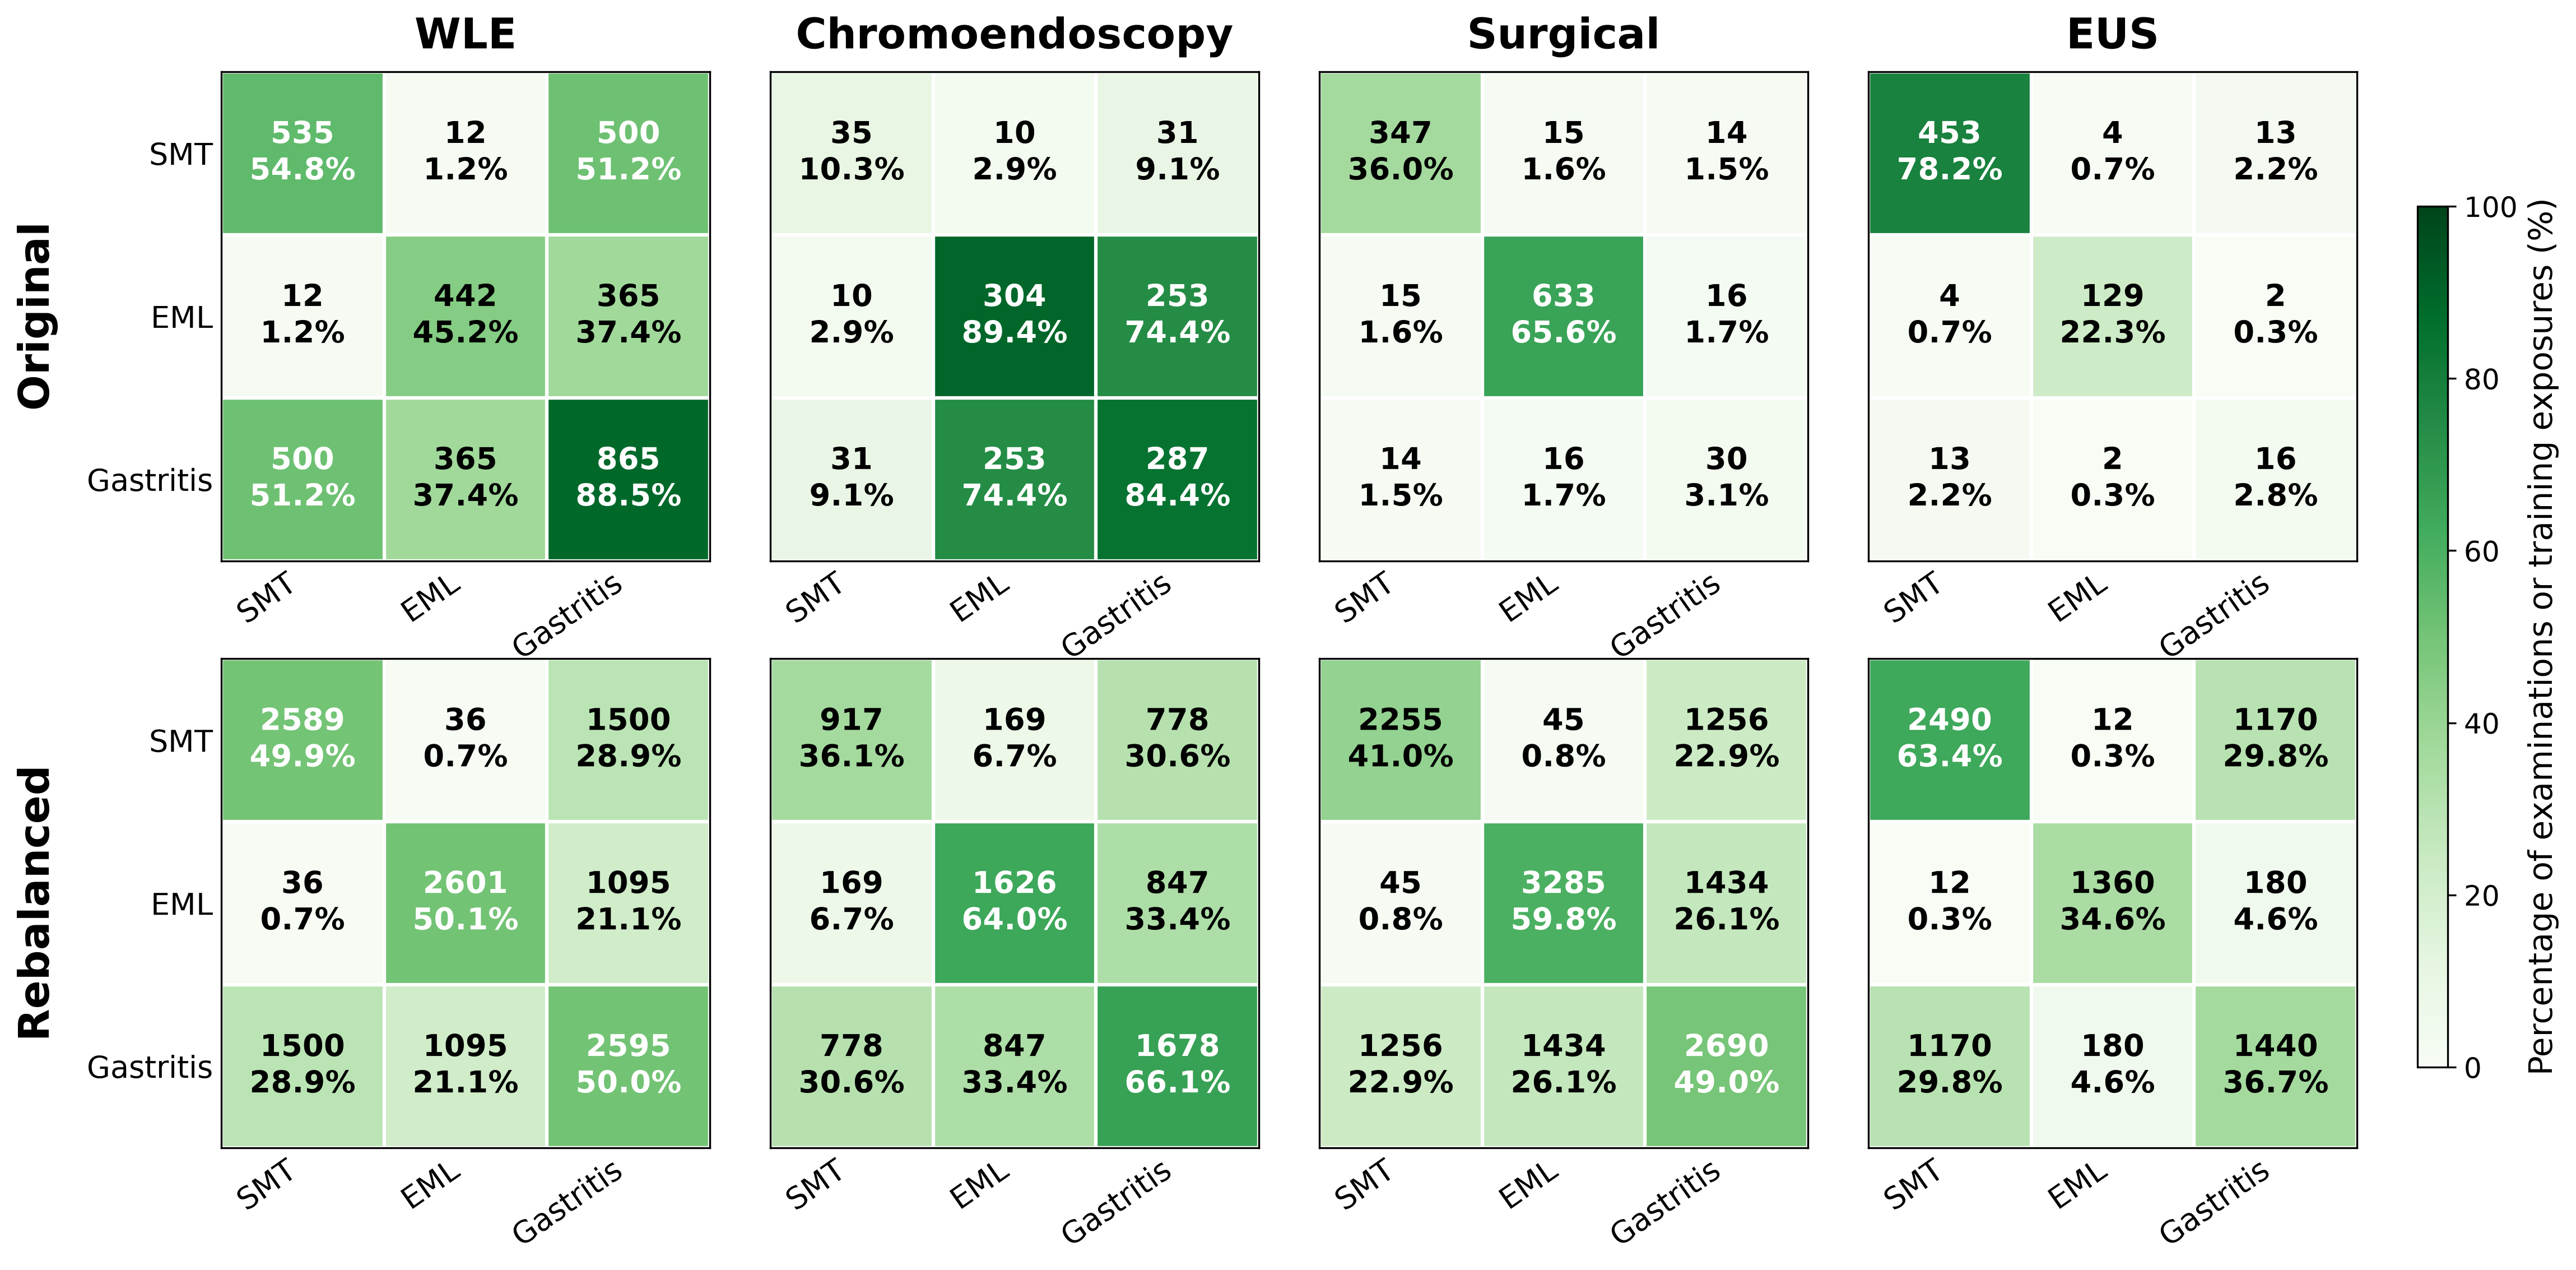
\includegraphics[width=\textwidth]{figs/label_cooccurrence_overview.png}
\caption{Original and rebalanced label co-occurrence matrices for the four gastroscopy datasets. Columns show the WLE, chromoendoscopy, surgical gastroscopy, and EUS distributions. The upper row presents the original examination distributions. The lower row presents the cumulative distribution obtained by pooling all five independently rebalanced training sets within each dataset; validation and test sets were not rebalanced or included. Each cell reports the corresponding count and percentage. Diagonal cells denote single-label positive frequencies, and off-diagonal cells denote pairwise co-positive frequencies. Percentages are calculated relative to the corresponding original dataset or pooled training exposures. SMT, esophageal submucosal tumor; EML, esophageal mucosal lesion.\label{fig:label_cooccurrence}}
\end{figure*}

\subsubsection{Examination-level multimodal sample construction}

Each eligible examination was represented by its complete ordered image sequence, a three-dimensional multi-label target, and the gastroscopic finding description text. For model preparation, at most $T=64$ images were uniformly sampled from each examination while preserving their original order. Each image was resized to 224$\times$224 pixels. A binary mask $M_i=\{m_{i1},\ldots,m_{iT}\}$ distinguished valid images from padded positions. The matched gastroscopic finding description text was retained as the text input; its category masking and encoding procedures are described in the text encoding section.

\subsection{Overview of AMEF-MIL}

As illustrated in Figure~\ref{fig:model_architecture}, AMEF-MIL organizes each examination as an ordered image bag, a valid-image mask, a finding description, and an examination-level multi-label target. The image branch applies a shared ConvNeXt-Tiny backbone and projection layer to obtain instance features. APro-CoPE preserves the original acquisition coordinates, constructs content-adaptive contextual coordinates, and delivers absolute and relative position signals to the bidirectional Transformer. Multi-label attention MIL then produces disease-specific visual representations, which the label hypergraph reasoner refines through higher-order interactions among coexisting findings. In parallel, category masking and a multi-scale TextCNN encode the finding description into token-level features. Each refined visual label representation retrieves disease-relevant textual evidence through label-wise cross-attention, and the gated residual module integrates the retrieved representation with its corresponding visual representation. The fused representations drive the primary multimodal branch, while the hypergraph-refined visual representations drive the auxiliary image-only branch. During training, ground-truth supervision jointly optimizes the two branches, and the pretrained multimodal teacher supplies prediction-level knowledge to the image-only branch. Figure~\ref{fig:apro_cope} further presents the mathematical construction of APro-CoPE.

\begin{figure*}[t]
\centering
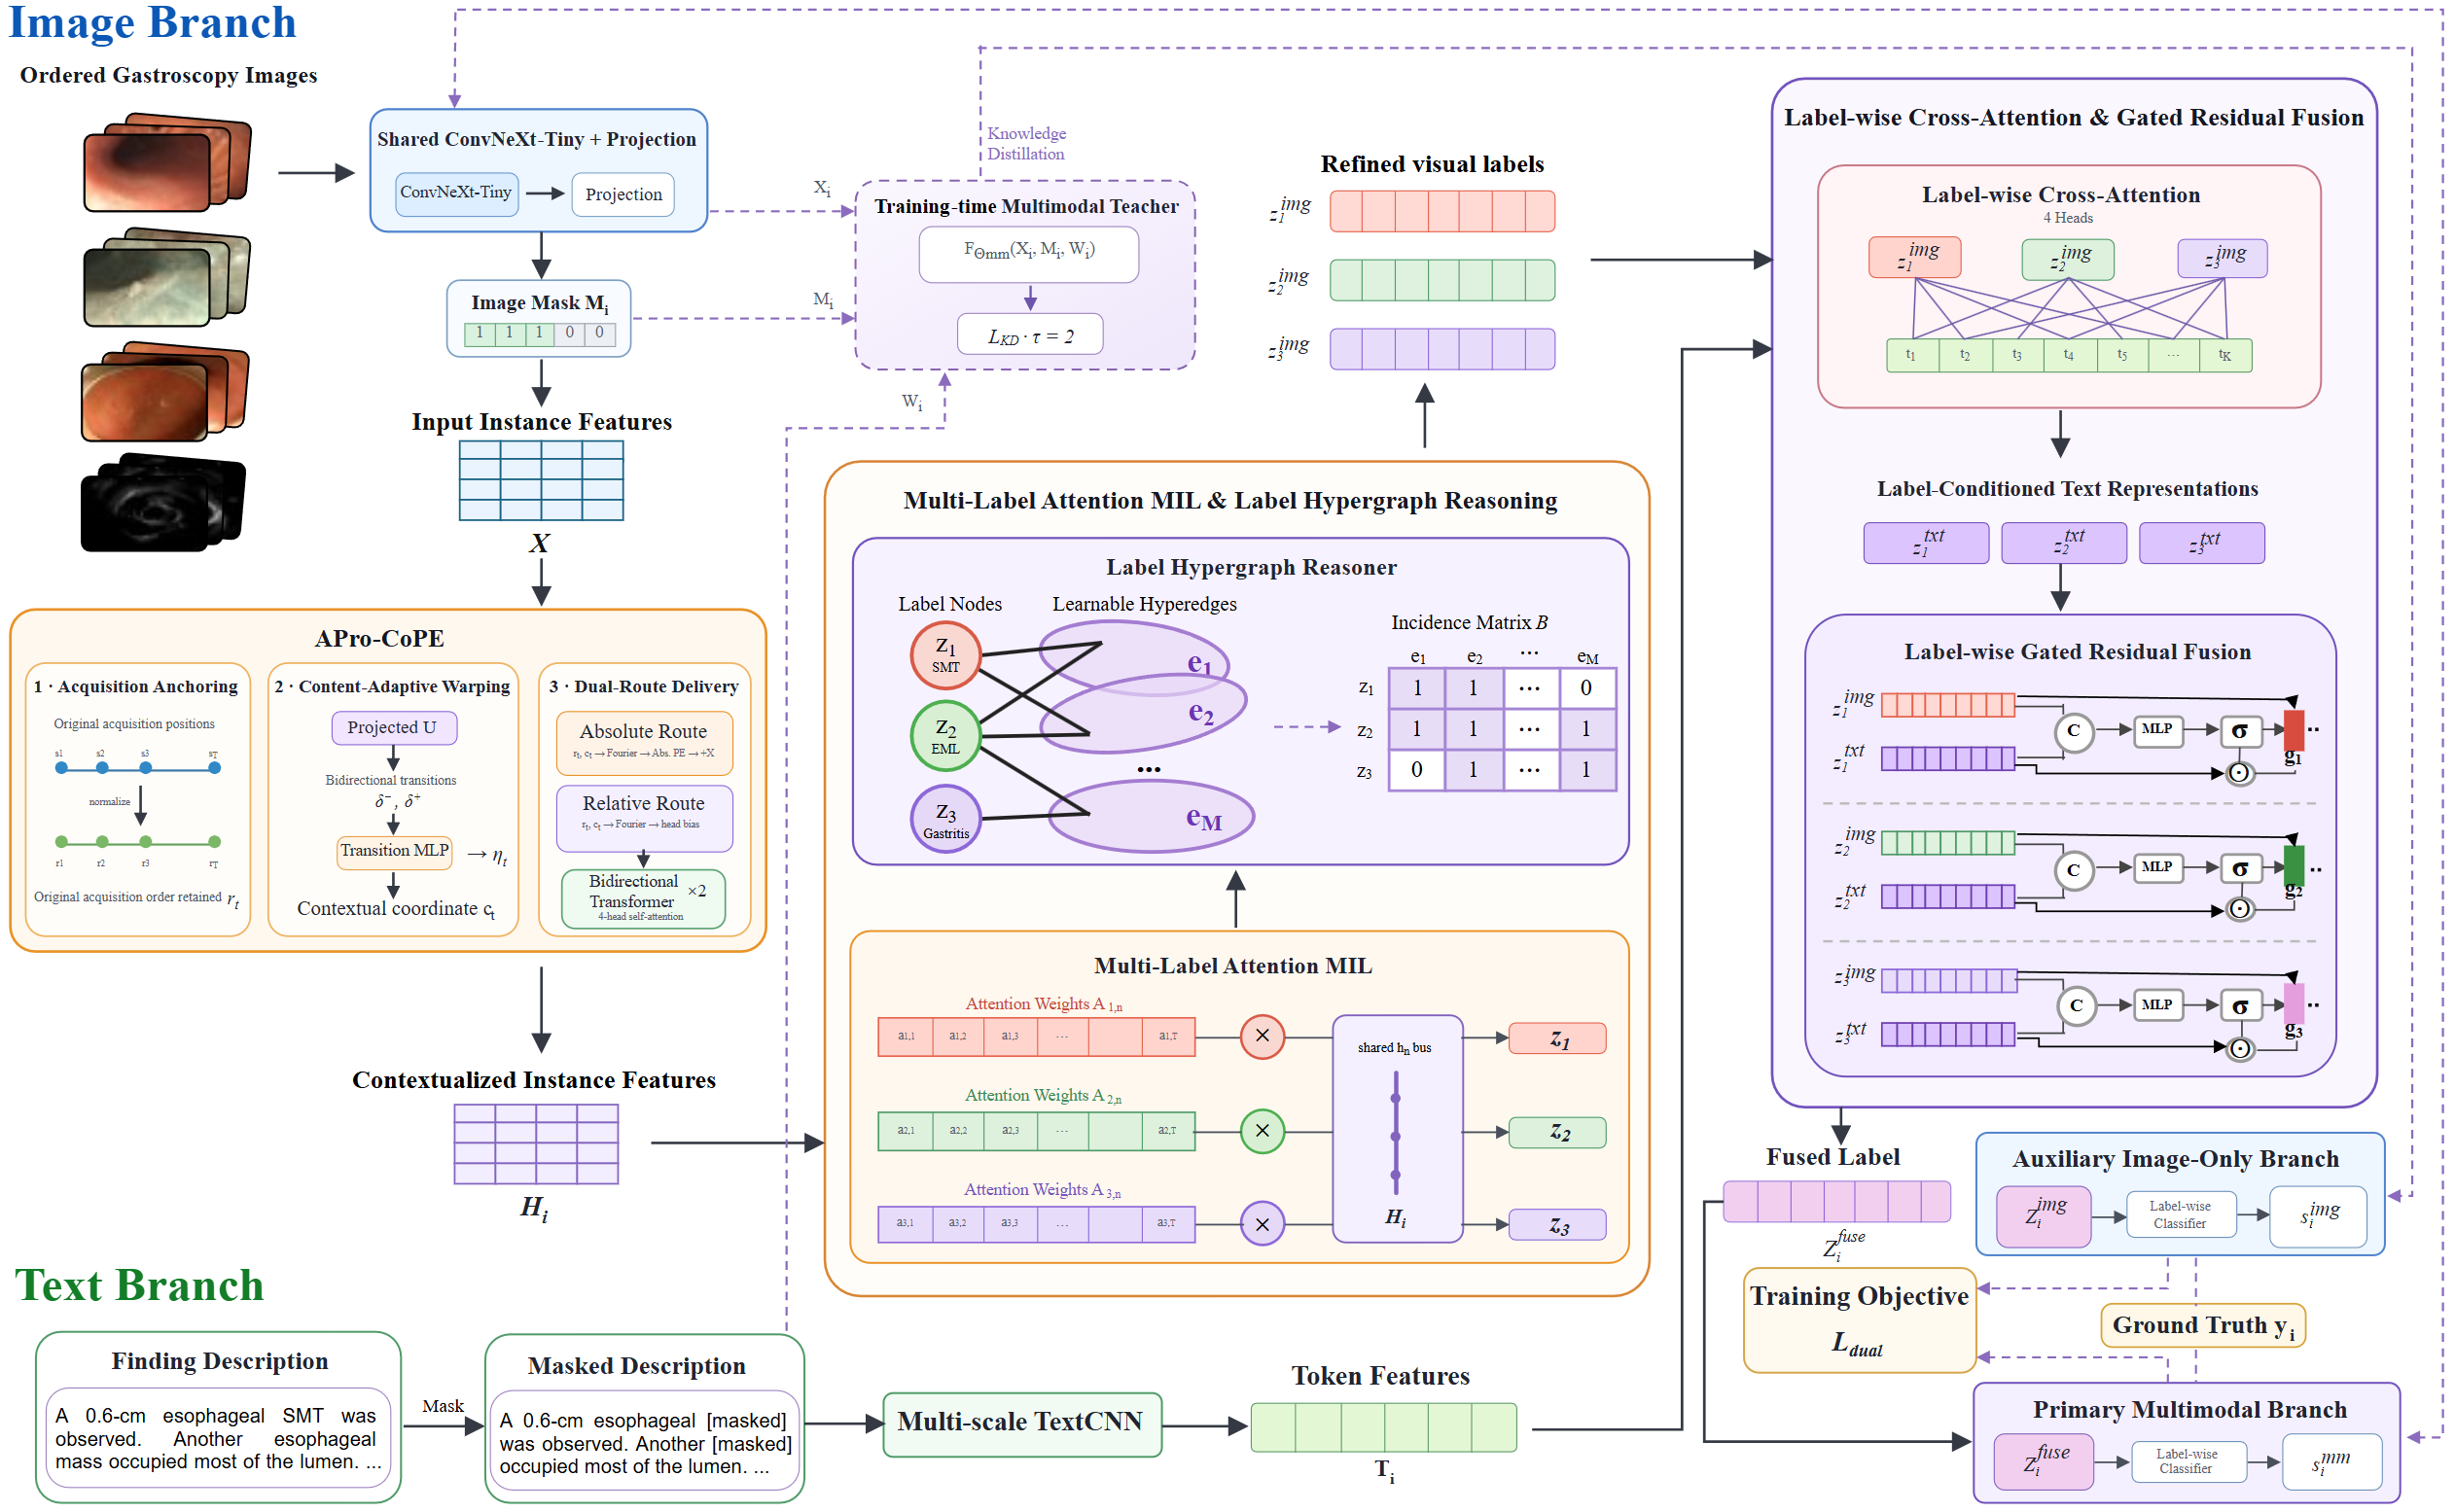
\includegraphics[width=\textwidth]{figs/amef_mil_overall_architecture.png}
\caption{Overall architecture of AMEF-MIL. The image branch combines shared visual encoding, APro-CoPE-based bidirectional context modeling, multi-label attention MIL, and label hypergraph reasoning. The text branch encodes category-masked finding descriptions with a multi-scale TextCNN. Label-wise cross-attention and gated residual fusion generate the primary multimodal prediction, while the hypergraph-refined visual representations support the auxiliary image-only prediction and receive training-time knowledge from the pretrained multimodal teacher.\label{fig:model_architecture}}
\end{figure*}

\subsection{Image Encoding}

For the $i$-th gastroscopy examination, let $X_i=\{I_{i1},I_{i2},\ldots,I_{iN_i}\}$ denote its variable-length image bag, $M_i$ the valid-image mask, and $y_i\in\{0,1\}^{L}$ the examination-level target, where $L=3$. The three dimensions correspond to esophageal submucosal tumor, esophageal mucosal lesion, and gastritis, and more than one label may be positive in the same examination. The image encoder maps $X_i$ and $M_i$ to label-specific visual representations that are subsequently used by both prediction branches.

\subsubsection{Image encoding and APro-CoPE procedural context modeling}

Each sampled image was encoded by a shared ConvNeXt-Tiny backbone followed by a projection head, producing a $d=512$ dimensional instance feature $x_{it}$.\cite{R28} A two-layer bidirectional Transformer supplied the intra-examination context backbone. Compared with conventional position encoding based on sampled-slot indices, we developed a more innovative Acquisition-Anchored Procedural Contextual Position Encoding (APro-CoPE). It was motivated by the context-dependent position increments of CoPE, but was reformulated for a non-causal clinical acquisition sequence with explicit acquisition anchors, monotonicity, and endpoint conservation. Figure~\ref{fig:apro_cope} summarizes its acquisition anchoring, contextual coordinate construction, and dual-route position delivery.

Let $s_{it}\in\{0,\ldots,N_i-1\}$ be the original index of the $t$-th sampled image in an examination containing $N_i$ acquired images. Its raw acquisition anchor is
\begin{equation}
r_{it}=\frac{s_{it}}{\max(N_i-1,1)}.
\end{equation}
Consequently, uniform or non-uniform subsampling does not replace the original procedural coordinate with a new slot coordinate. We projected the visual feature as $u_{it}=\operatorname{LN}(W_px_{it})$ and formed backward and forward transitions $\delta^-_{it}=u_{it}-u_{i,t-1}$ and $\delta^+_{it}=u_{i,t+1}-u_{it}$. A persistent transition score was then estimated from the current feature, the two signed transitions, their magnitudes, their element-wise agreement, and the raw acquisition gap:
\begin{equation}
\begin{aligned}
\eta_{it}={}&\alpha\tanh\!\Bigl(\operatorname{MLP}\!\bigl(
[u_{it},\delta^-_{it},\delta^+_{it},\\
&|\delta^-_{it}|,|\delta^+_{it}|,
\delta^-_{it}\odot\delta^+_{it},\Delta r_{it}]\bigr)\Bigr),
\end{aligned}
\end{equation}
where $\Delta r_{it}=r_{it}-r_{i,t-1}$ and $\alpha=1.5$ bounds the deformation magnitude. The contextual gap and coordinate were defined as
\begin{align}
g_{it}&=\Delta r_{it}\exp(\eta_{it}),\\
\widetilde g_{it}&=\frac{(r_{iT_i}-r_{i1})g_{it}}{\sum_{k=2}^{T_i}g_{ik}},\\
c_{i1}&=r_{i1},\qquad c_{it}=r_{i1}+\sum_{k=2}^{t}\widetilde g_{ik},
\end{align}
where $T_i$ is the number of valid sampled images. Because every warped gap is positive and the gaps are renormalized to the observed acquisition span, $c_{it}$ remains monotonic and preserves both sequence endpoints.

APro-CoPE delivers position information through two complementary routes. The absolute route adds
\begin{equation}
\begin{aligned}
p^{\mathrm{abs}}_{it}={}&f_{\mathrm{abs}}([\phi(r_{it}),\phi(c_{it}),\\
&\phi(c_{it}-r_{it})])
\end{aligned}
\end{equation}
to $x_{it}$, where $\phi(\cdot)$ is an eight-frequency continuous Fourier mapping. The relative route generates a head-specific attention bias
\begin{equation}
\begin{aligned}
b^{(h)}_{itu}={}&2\tanh f^{(h)}_{\mathrm{rel}}\bigl([\phi(r_{it}-r_{iu}),
\phi(c_{it}-c_{iu}),\\
&\phi((c_{it}-c_{iu})-(r_{it}-r_{iu}))]\bigr).
\end{aligned}
\end{equation}
The resulting features were processed by the two-layer, four-head bidirectional Transformer, with $b^{(h)}_{itu}$ added to the scaled dot-product attention logits. The valid-image mask excluded padded positions throughout, producing $H_i=\{h_{i1},\ldots,h_{iT_i}\}\in\mathbb{R}^{T_i\times d}$.

\begin{figure*}[t]
\centering
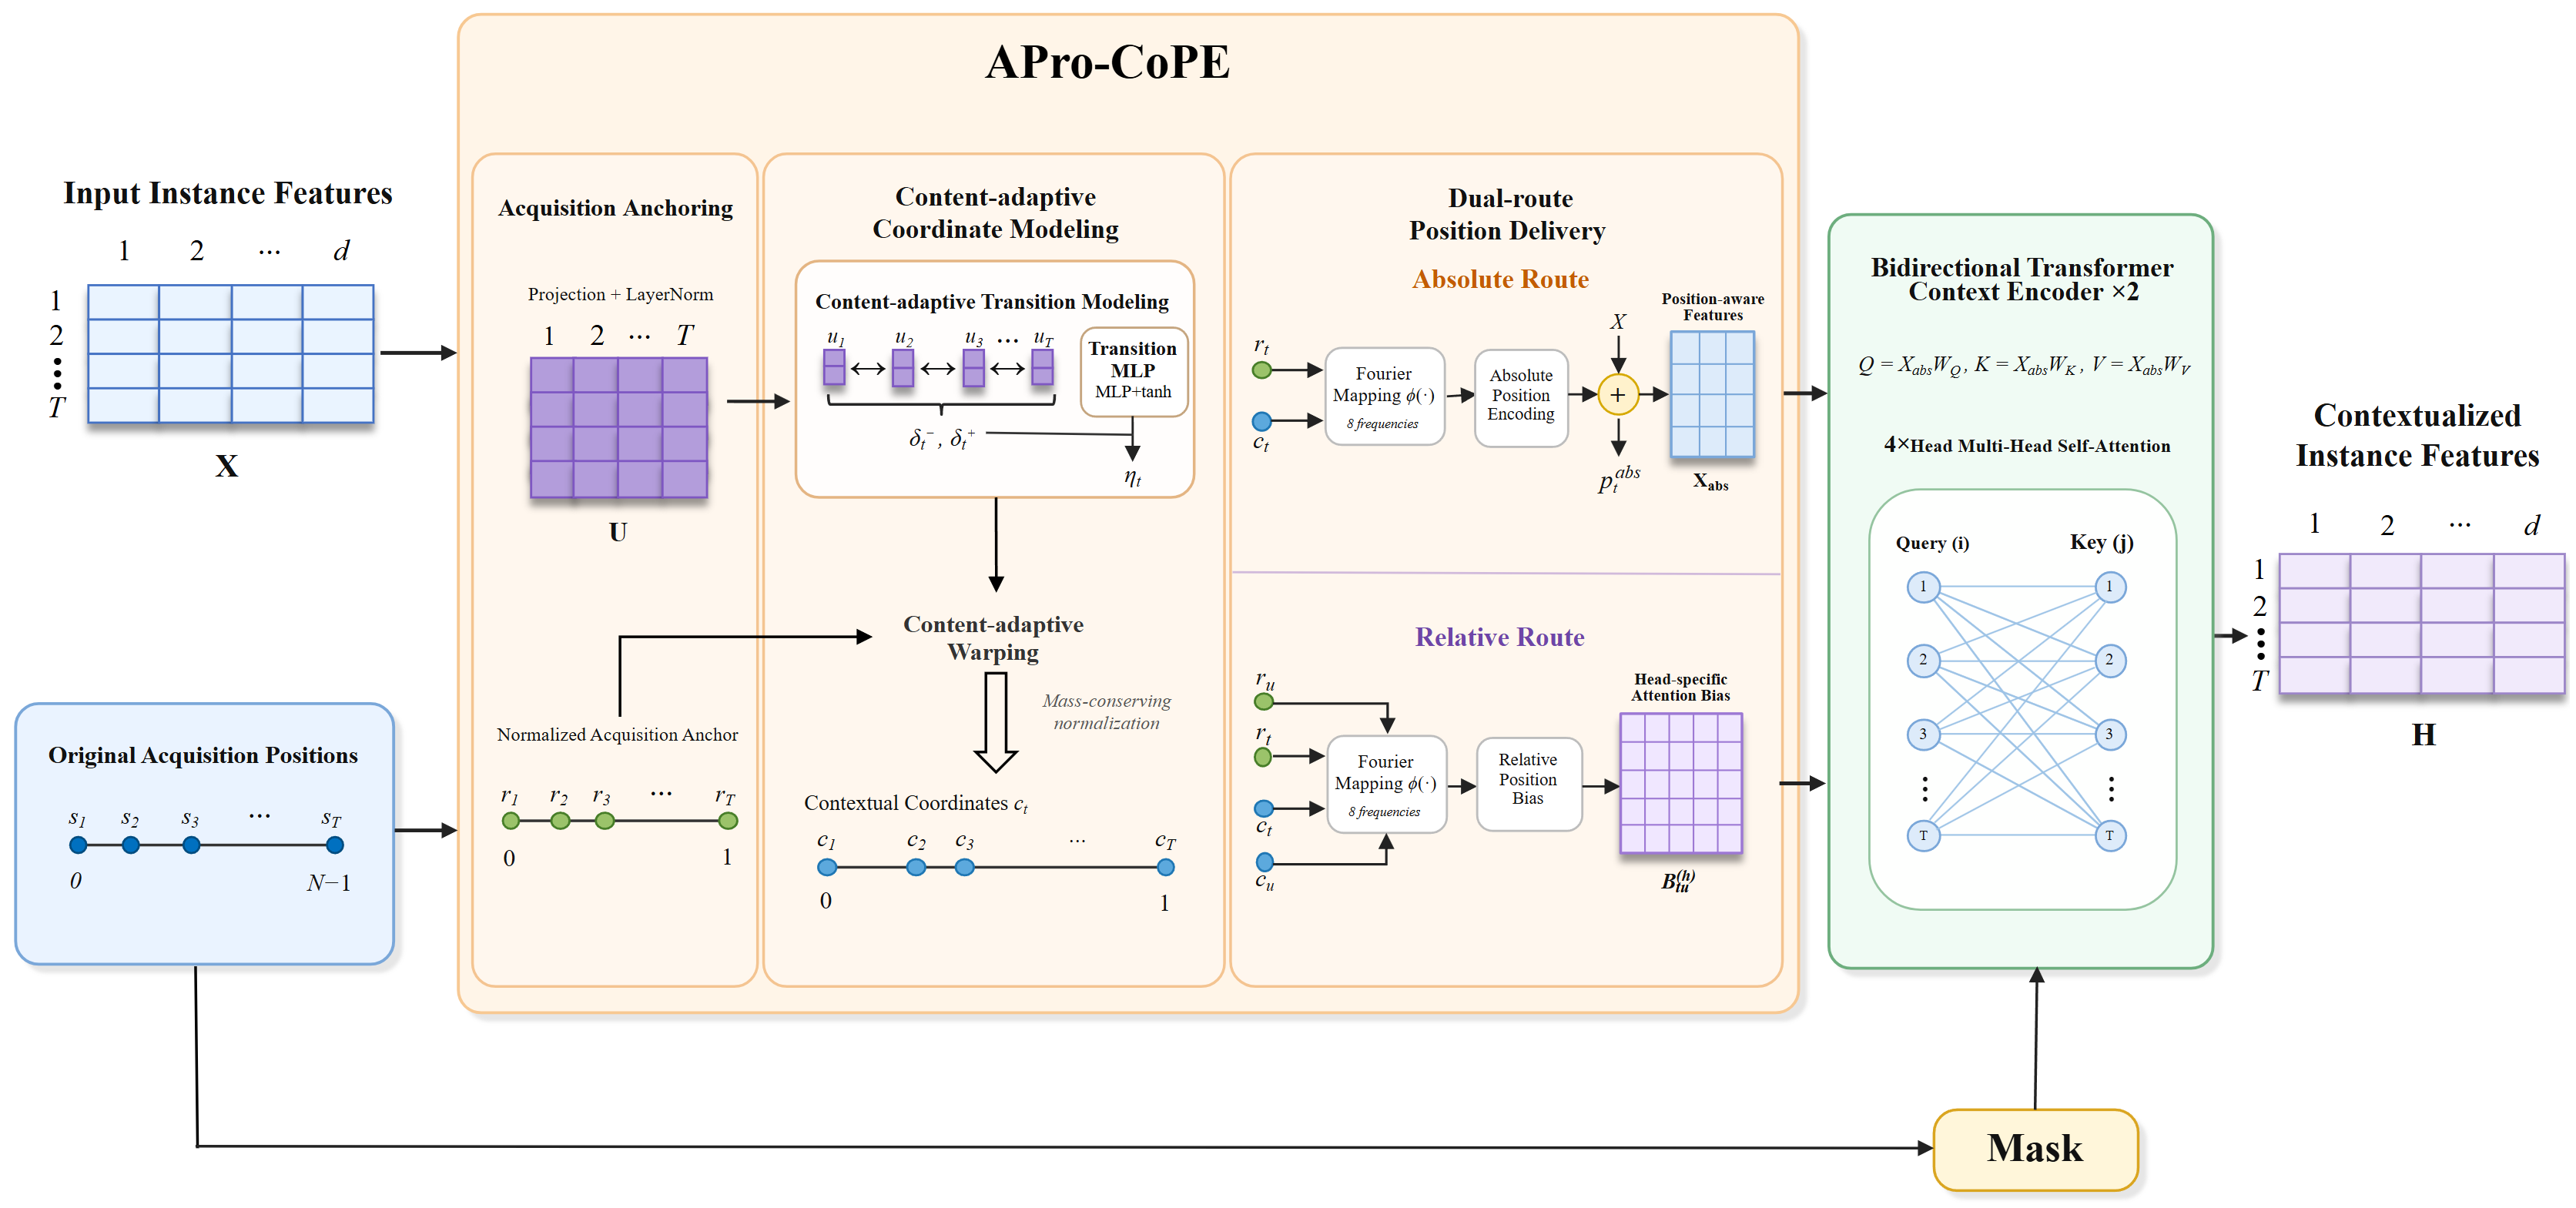
\includegraphics[width=\textwidth]{figs/apro_cope_bidirectional_transformer.png}
\caption{Structure of APro-CoPE. Original acquisition indices define normalized acquisition anchors. Bidirectional visual transitions are used to estimate bounded contextual deformation scores, and mass-conserving normalization constructs a monotonic contextual coordinate while preserving the observed sequence endpoints. The absolute route augments the instance features, whereas the relative route provides head-specific attention biases to the bidirectional Transformer.\label{fig:apro_cope}}
\end{figure*}

\subsubsection{Multi-label attention MIL}

Different diseases may be supported by different images in the same examination. The model therefore learned one gated attention distribution for each label. For image $n$, the shared gated attention feature was
\begin{equation}
q_{in}=\tanh(Vh_{in})\odot\sigma(Uh_{in}),
\end{equation}
and the attention score and normalized weight for label $\ell$ were
\begin{equation}
\begin{aligned}
e_{i\ell n}&=w_{\ell}^{\top}q_{in},\\
a_{i\ell n}&=\frac{m_{in}\exp(e_{i\ell n})}
{\sum_{t=1}^{T}m_{it}\exp(e_{i\ell t})+\epsilon}.
\end{aligned}
\end{equation}
The label-specific visual representation was obtained as
\begin{equation}
z_{i\ell}=\sum_{n=1}^{T}a_{i\ell n}h_{in}.
\end{equation}
This operation allows each disease to aggregate its own supporting images while ignoring invalid positions.

\subsubsection{Label hypergraph reasoning}

Let $Z_i=[z_{i1},\ldots,z_{iL}]^{\top}\in\mathbb{R}^{L\times d}$ denote the label-specific visual feature matrix. To model higher-order relationships among coexisting diseases, the label hypergraph reasoner learned an incidence matrix $B\in\mathbb{R}^{L\times E}$ with $E=2$ latent hyperedges. After normalization, information was propagated from label nodes to hyperedges and then back to label nodes:
\begin{equation}
U_i=S_{node\rightarrow edge}^{\top}\eta(Z_i),
\end{equation}
\begin{equation}
\widetilde{Z}_i=S_{edge\rightarrow node}U_i,
\end{equation}
\begin{equation}
Z_i^{img}=Z_i+\phi([Z_i;\widetilde{Z}_i]),
\end{equation}
where $\eta(\cdot)$ and $\phi(\cdot)$ are learnable transformations. The resulting $Z_i^{img}$ retains one hypergraph-refined visual representation for each disease and serves as the visual input to both prediction branches.

\subsection{Text Encoding}

\subsubsection{Finding-description selection and category masking}

The text encoder used the gastroscopic finding description text. This text describes lesion morphology, location, and surrounding mucosal changes, but it may also directly contain a target category name. To reduce direct label leakage, canonical disease names, abbreviations, and direct lexical variants associated with the three targets were replaced with a common mask token before tokenization. The masking lexicon covered direct category expressions such as esophageal submucosal tumor or SMT, esophageal mucosal lesion, and named forms of gastritis, while retaining anatomical locations and descriptive morphology. The same masking procedure was applied to all data subsets.

\subsubsection{TextCNN-based finding-description encoding}

After category masking, whitespace and punctuation were normalized, and each finding description $W_i$ was tokenized into Chinese characters and alphanumeric fragments. The resulting tokens were mapped deterministically to a fixed vocabulary of 8192 indices and converted into 128-dimensional embeddings. Finding descriptions were truncated or padded to a maximum length of $K=128$, with a binary text mask identifying valid token positions. Let $E_i\in\mathbb{R}^{K\times128}$ denote the embedded token sequence. A multi-scale TextCNN applied parallel one-dimensional convolutions with kernel sizes $r\in\{2,3,4\}$ and same-length padding:
\begin{equation}
H_i^{(r)}=\mathrm{ReLU}\!\left(\mathrm{Conv1D}_{r}(E_i)\right),
\qquad r\in\{2,3,4\}.
\end{equation}
The multi-scale features were concatenated, normalized, and projected into the same $d=512$ dimensional space as the visual features:
\begin{equation}
\begin{aligned}
T_i={}&\mathrm{Dropout}\!\Bigl(\mathrm{GELU}\!\bigl(
W_t\,\mathrm{LN}\!\left([H_i^{(2)};H_i^{(3)};H_i^{(4)}]\right)\\
&\qquad+b_t\bigr)\Bigr)\in\mathbb{R}^{K\times d}.
\end{aligned}
\end{equation}
Padding positions in $T_i$ were suppressed by the text mask, and the valid token-level representations were retained for label-query cross-attention. The embedding, convolutional, and projection parameters were optimized jointly with the complete model.

\subsection{Cross-Modal Fusion}

\subsubsection{Label-query cross-attention and gated fusion}

The visual and textual representations encode complementary forms of evidence at different granularities: $Z_i^{img}\in\mathbb{R}^{L\times d}$ contains one examination-level representation for each disease, whereas $T_i\in\mathbb{R}^{K\times d}$ retains token-level finding-description information. Directly pooling $T_i$ into a single vector would force all labels to share the same textual summary. We therefore used each hypergraph-refined visual label representation $z_{i\ell}^{img}$ as a query and the finding-description tokens as keys and values. For attention head $h\in\{1,\ldots,H\}$, where $H=4$ and $d_h=d/H$, the projected query, key, and value were
\begin{equation}
\begin{aligned}
q_{i\ell}^{(h)}&=(z_{i\ell}^{img}+u_{\ell})W_Q^{(h)},\qquad
k_{ik}^{(h)}=t_{ik}W_K^{(h)},\\
v_{ik}^{(h)}&=t_{ik}W_V^{(h)},
\end{aligned}
\end{equation}
where $u_{\ell}\in\mathbb{R}^{d}$ is a learnable label-identity embedding that preserves the distinction among disease queries during textual retrieval.
Let $\mu_{ik}\in\{0,1\}$ indicate whether the $k$-th textual position is valid. The label-to-token attention scores and normalized weights were calculated as
\begin{equation}
\begin{aligned}
e_{i\ell k}^{(h)}&=\frac{q_{i\ell}^{(h)}{k_{ik}^{(h)}}^{\top}}{\sqrt{d_h}},\\
\alpha_{i\ell k}^{(h)}&=
\frac{\mu_{ik}\exp(e_{i\ell k}^{(h)})}
{\sum_{u=1}^{K}\mu_{iu}\exp(e_{i\ell u}^{(h)})+\epsilon}.
\end{aligned}
\end{equation}
Thus, invalid padding positions did not participate in retrieval, and each disease label learned an independent attention distribution over the same finding description. The head-specific textual context and the resulting label-conditioned text representation were
\begin{equation}
\begin{aligned}
o_{i\ell}^{(h)}&=\sum_{k=1}^{K}\alpha_{i\ell k}^{(h)}v_{ik}^{(h)},\\
z_{i\ell}^{txt}&=\operatorname{Concat}_{h=1}^{H}\!\left(o_{i\ell}^{(h)}\right)W_O.
\end{aligned}
\end{equation}
Stacking the representations of all labels gives $Z_i^{txt}\in\mathbb{R}^{L\times d}$. This construction preserves label correspondence during fusion: the visual evidence for label $\ell$ retrieves textual evidence specifically for the same prediction rather than using a finding-description representation shared indiscriminately by all labels.

Because the relevance and reliability of the retrieved text can differ across diseases and examinations, a scalar gate was estimated separately for each label:
\begin{equation}
g_{i\ell}=a_i\,\sigma\!\left(\rho([z_{i\ell}^{img};z_{i\ell}^{txt}])\right),
\end{equation}
where $\rho(\cdot)$ is a two-layer multilayer perceptron and $a_i\in\{0,1\}$ indicates whether the examination contains valid finding-description text. The fused representation was formed through gated residual injection:
\begin{equation}
z_{i\ell}^{fuse}=z_{i\ell}^{img}+g_{i\ell}z_{i\ell}^{txt}.
\end{equation}
The residual form preserves the visual representation while allowing the model to introduce label-relevant semantic evidence with an examination- and label-dependent magnitude. When no valid finding-description text was available, $a_i=0$ and $z_{i\ell}^{fuse}=z_{i\ell}^{img}$.

To explicitly constrain label--text correspondence, we further introduced a label-query discrimination loss. For a positive label $\ell$ and an absent label $r$, let $\widetilde{s}_{i\ell\leftarrow r}^{mm}$ denote the counterfactual logit obtained by replacing $z_{i\ell}^{txt}$ with $z_{ir}^{txt}$ while retaining the visual representation, gate, and classifier of label $\ell$. The valid comparison set was $\mathcal{P}_i=\{(\ell,r)\mid a_i=1,\ y_{i\ell}=1,\ y_{ir}=0,\ \ell\neq r\}$. The loss was defined as
\begin{equation}
\begin{aligned}
\mathcal{L}_{LQD}={}&-\frac{1}{\sum_i|\mathcal{P}_i|}
\sum_i\sum_{(\ell,r)\in\mathcal{P}_i}\Big[
\log\sigma(s_{i\ell}^{mm})\\
&+\log\left(1-\sigma(\widetilde{s}_{i\ell\leftarrow r}^{mm})\right)\Big].
\end{aligned}
\end{equation}
This objective encourages the text retrieved by the matched query to support its positive disease prediction while preventing text retrieved by an absent disease query from acting as interchangeable evidence. Pairs of coexisting positive labels were excluded so that the constraint did not suppress clinically valid co-occurrence information.

\subsection{Prediction Branches}

\subsubsection{Primary multimodal branch}

Let $Z_i^{fuse}=[z_{i1}^{fuse},\ldots,z_{iL}^{fuse}]^{\top}$ denote the label-wise fused representation. The primary multimodal branch applied a label-wise classifier to this representation:
\begin{equation}
s_i^{mm}=C_{mm}(Z_i^{fuse}).
\end{equation}
Its parameters, together with the shared image encoder, text encoder, and cross-modal fusion modules, were optimized using examination-level asymmetric loss:
\begin{equation}
\mathcal{L}_{mm}=\mathcal{L}_{ASL}(s_i^{mm},y_i)+\lambda_q\mathcal{L}_{LQD}.
\end{equation}
Here, $\lambda_q$ controls the label-query discrimination constraint.
This branch constitutes the primary prediction pathway and uses both the endoscopic image sequence and the category-masked gastroscopic finding description.

For knowledge transfer to the image-only branch, a multimodal model with the same pathway was first pretrained using $\mathcal{L}_{mm}$. Its selected parameters were then fixed and denoted by $\overline{\Theta}_{mm}$. Given the same examination, the frozen teacher produced logits
\begin{equation}
\overline{s}_i^{mm}=F_{\overline{\Theta}_{mm}}(X_i,M_i,W_i),
\end{equation}
where $W_i$ denotes the category-masked finding description. The frozen teacher supplied soft targets but received no gradient during subsequent image-only training.

\subsubsection{Image-only branch and multimodal knowledge transfer}

The auxiliary image-only branch predicted directly from the hypergraph-refined visual representations:
\begin{equation}
s_i^{img}=C_{img}(Z_i^{img}).
\end{equation}
Its basic supervision used the same examination-level targets:
\begin{equation}
\mathcal{L}_{img}=\mathcal{L}_{ASL}(s_i^{img},y_i).
\end{equation}
When the trainable multimodal branch was supervised jointly, $\mathcal{L}_{mm}$ also updated the shared visual encoder and thereby provided an indirect representation-level learning signal to the image-only pathway.

Knowledge distillation provided a separate prediction-level transfer signal from the frozen multimodal teacher. With temperature $\tau$, the teacher probability and multi-label distillation loss were defined as
\begin{equation}
\overline{p}_i^{mm}=\sigma\!\left(\frac{\overline{s}_i^{mm}}{\tau}\right),
\end{equation}
\begin{equation}
\begin{aligned}
\mathcal{L}_{KD}={}&\tau^2\operatorname{BCEWithLogits}\!\left(
\frac{s_i^{img}}{\tau},\right.\\
&\left.\operatorname{sg}(\overline{p}_i^{mm})\right),
\end{aligned}
\end{equation}
where $\operatorname{sg}(\cdot)$ stops gradients through the teacher target. The joint objective was expressed as
\begin{equation}
\begin{aligned}
\mathcal{L}_{dual}={}&\mathcal{L}_{img}+\lambda_{mm}\mathcal{L}_{mm}\\
&+\lambda_{KD}\mathcal{L}_{KD},
\end{aligned}
\end{equation}
where $\lambda_{mm}$ and $\lambda_{KD}$ control the contributions of multimodal branch supervision and frozen-teacher distillation, respectively. At image-only inference, only $X_i$, $M_i$, and $C_{img}$ are required; the finding-description encoder, cross-modal fusion modules, and frozen teacher are not used.

\section{Experiments}

\subsection{Experimental Settings}

All experiments followed the patient-grouped five-fold protocol described above and used random seed 2026. Models were trained for at most 30 epochs with AdamW, an initial learning rate of $2\times10^{-5}$, a weight decay of 0.02, and an examination-level batch size of 1. Gradients were accumulated over four examinations. The learning rate was linearly warmed up during the first 20\% of optimization steps and then decayed following a cosine schedule. Automatic mixed precision was enabled, dropout was set to 0.2, and asymmetric loss was used for multi-label supervision. The experiments were executed as independent fold-level jobs on six NVIDIA GeForce RTX 4090 GPUs.

For image encoding, input images were resized to 224$\times$224 pixels and processed by a pretrained ConvNeXt-Tiny with its first stage frozen. Unless otherwise specified, up to 64 images were uniformly sampled from each examination, and the projected feature dimension was 512. The context encoder contained two bidirectional Transformer layers with four attention heads, and the label hypergraph contained two latent hyperedges. Full APro-CoPE used a 64-dimensional transition space, eight Fourier frequencies, $\alpha=1.5$, mass conservation, and both absolute and relative position routes. For text encoding, finding descriptions were limited to 128 tokens and represented using a vocabulary of 8192 indices, 128-dimensional embeddings, and TextCNN kernels of sizes 2, 3, and 4. Label-query cross-attention used four heads, followed by label-wise gated residual fusion, and the label-query discrimination weight was $\lambda_q=0.01$. The primary multimodal output used the endoscopic image sequence and category-masked gastroscopic finding description. In the image-only transfer experiments, the auxiliary image-only classification loss had a weight of 0.5; the distillation-loss weight was set to 0 or 1, and the temperature was $\tau=2$.

Macro F1 was used as the primary evaluation and model-selection metric because it assigns equal importance to all three target labels under class imbalance. The checkpoint with the highest validation macro F1 was selected for each fold, and the final results are reported as the mean and standard deviation across the five patient-grouped folds. All experimental comparisons passed statistical significance testing.

\subsection{Overall Performance Comparison and Label-wise Analysis}

\subsubsection{Comparison with image-only, text-only, and multimodal models}

To evaluate overall examination-level classification performance, we compared AMEF-MIL with image-only MIL methods, text-only encoders, and multimodal classification models under the same patient-grouped five-fold protocol. The four multimodal comparison methods were reimplemented by adapting their fusion mechanisms to examination-level image bags and category-masked gastroscopic finding descriptions while retaining the common data splits and optimization settings.\cite{R29,R30,R31,R32}

Table~\ref{T2} presents the comparison results. AMEF-MIL achieved the highest mean macro F1 on all four datasets: 0.9149 on WLE, 0.8877 on chromoscopic gastroscopy, 0.8456 on surgical gastroscopy, and 0.9064 on EUS. In every dataset, AMEF-MIL outperformed the strongest image-only model and the strongest text-only model. This provides direct evidence that the model forms an effective multimodal representation by integrating the complementary discriminative information contributed by the ordered image sequence and the category-masked finding description. AMEF-MIL also outperformed all selected multimodal baselines across the four datasets, demonstrating the advantage of the complete pipeline---acquisition-aware image encoding, label hypergraph reasoning, disease-specific cross-attention, and gated residual fusion---for examination-level multi-label classification. This advantage was most pronounced on chromoscopic gastroscopy, where AMEF-MIL achieved both the highest mean macro F1 and the lowest fold-to-fold standard deviation among all compared methods.

\begin{table*}[t]
\scriptsize\tabletimes\centering
\caption{Comparison with image-only, text-only, and multimodal methods across the four gastroscopy datasets. Values are macro F1 reported as mean $\pm$ standard deviation over five patient-grouped folds. img. and txt. denote endoscopic image and category-masked gastroscopic finding description inputs, respectively.\label{T2}}
\resizebox{\textwidth}{!}{%
\begin{tabular}{lcc*{4}{c}}
\hline
Model & img. & txt. & WLE & Chromoscopic & Surgical & EUS \\
\hline
Attention MIL & $\checkmark$ & $\times$ & \tresult{0.7919}{0.0119} & \tresult{0.7391}{0.0448} & \tresult{0.7018}{0.1235} & \tresult{0.6268}{0.0342} \\
Mean pooling & $\checkmark$ & $\times$ & \tresult{0.7931}{0.0088} & \tresult{0.7408}{0.0322} & \tresult{0.7173}{0.0744} & \tresult{0.5910}{0.0592} \\
Transformer-context MIL & $\checkmark$ & $\times$ & \tresult{0.8004}{0.0160} & \tresult{0.7426}{0.0194} & \tresult{0.7765}{0.0886} & \tresult{0.5966}{0.0612} \\
Top-$k$ MIL & $\checkmark$ & $\times$ & \tresult{0.7862}{0.0232} & \tresult{0.7511}{0.0406} & \tresult{0.7698}{0.0849} & \tresult{0.6037}{0.0887} \\
Max pooling & $\checkmark$ & $\times$ & \tresult{0.7608}{0.0034} & \tresult{0.6842}{0.0261} & \tresult{0.6009}{0.0919} & \tresult{0.5505}{0.0756} \\
TransMIL & $\checkmark$ & $\times$ & \tresult{0.8021}{0.0146} & \tresult{0.7217}{0.0368} & \tresult{0.7516}{0.0938} & \tresult{0.6045}{0.0539} \\
DSMIL & $\checkmark$ & $\times$ & \tresult{0.7956}{0.0159} & \tresult{0.7468}{0.0448} & \tresult{0.6873}{0.0852} & \tresult{0.5765}{0.0765} \\
DTFD-MIL & $\checkmark$ & $\times$ & \tresult{0.7714}{0.0141} & \tresult{0.7091}{0.0306} & \tresult{0.7134}{0.0853} & \tresult{0.5896}{0.0419} \\
CLAM-MB & $\checkmark$ & $\times$ & \tresult{0.7741}{0.0090} & \tresult{0.7137}{0.0269} & \tresult{0.7094}{0.0865} & \tresult{0.5883}{0.0401} \\
CLAM-SB & $\checkmark$ & $\times$ & \tresult{0.7642}{0.0040} & \tresult{0.6997}{0.0234} & \tresult{0.6785}{0.0479} & \tresult{0.5695}{0.0379} \\
\hline
Hashed mean & $\times$ & $\checkmark$ & \tresult{0.8901}{0.0184} & \tresult{0.8037}{0.0689} & \tresult{0.8349}{0.0187} & \tresult{0.8836}{0.0688} \\
Vocabulary attention & $\times$ & $\checkmark$ & \tresult{0.8906}{0.0124} & \tresult{0.8045}{0.0708} & \tresult{0.8147}{0.0487} & \tresult{0.8957}{0.0542} \\
TextCNN & $\times$ & $\checkmark$ & \tresult{0.9004}{0.0123} & \tresult{0.8652}{0.0332} & \tresult{0.8356}{0.0807} & \tresult{0.8982}{0.0515} \\
BiGRU & $\times$ & $\checkmark$ & \tresult{0.8928}{0.0191} & \tresult{0.8085}{0.0818} & \tresult{0.8075}{0.0342} & \tresult{0.9019}{0.0531} \\
Transformer & $\times$ & $\checkmark$ & \tresult{0.8915}{0.0163} & \tresult{0.8150}{0.0281} & \tresult{0.8285}{0.0174} & \tresult{0.8830}{0.0604} \\
\hline
MMFNet (2024)\cite{R29}$^{\dagger}$ & $\checkmark$ & $\checkmark$ & \tresult{0.9132}{0.0099} & \tresult{0.8371}{0.0647} & \tresult{0.8345}{0.0844} & \tresult{0.8999}{0.0731} \\
RadFuse (2025)\cite{R32}$^{\dagger}$ & $\checkmark$ & $\checkmark$ & \tresult{0.9135}{0.0083} & \tresult{0.7990}{0.1013} & \tresult{0.8221}{0.0671} & \tresult{0.8517}{0.0712} \\
SAIF (2025)\cite{R30}$^{\dagger}$ & $\checkmark$ & $\checkmark$ & \tresult{0.8413}{0.0166} & \tresult{0.7201}{0.0544} & \tresult{0.7482}{0.0821} & \tresult{0.6266}{0.0986} \\
MMTF (2026)\cite{R31}$^{\dagger}$ & $\checkmark$ & $\checkmark$ & \tresult{0.9121}{0.0118} & \tresult{0.7320}{0.0415} & \tresult{0.7595}{0.1371} & \tresult{0.7846}{0.0974} \\
\hline
AMEF-MIL (Ours) & $\checkmark$ & $\checkmark$ & \tresult{\textbf{0.9149}}{\textbf{0.0114}} & \tresult{\textbf{0.8877}}{\textbf{0.0168}} & \tresult{\textbf{0.8456}}{\textbf{0.0224}} & \tresult{\textbf{0.9064}}{\textbf{0.0474}} \\
\hline
\end{tabular}
}
\par\raggedright\scriptsize $^{\dagger}$Reimplemented using the same examination-level inputs, category-masking procedure, patient-grouped folds, and optimization protocol as AMEF-MIL.
\end{table*}

\subsubsection{Out-of-fold label-wise confusion analysis}

Figure~\ref{fig:oof_confusion_selected} further examines label-wise decisions by pooling predictions from the five mutually exclusive test folds, so each eligible examination contributes exactly once. Separate one-vs-rest $2\times2$ confusion matrices are reported because each examination may contain more than one positive label.

Positive-class sensitivity was high for most dataset--label combinations, including 97.9\% for esophageal submucosal tumor and 97.7\% for gastritis in WLE, 99.0\% for esophageal mucosal lesion in chromoscopic gastroscopy, 94.5\% for esophageal submucosal tumor in surgical gastroscopy, and 99.6\% for esophageal submucosal tumor in EUS. The principal errors were false-positive predictions for labels with relatively few negative examinations, most visibly esophageal mucosal lesion and gastritis in chromoscopic gastroscopy and gastritis in WLE. These patterns complement macro F1 by showing how label prevalence and the selected decision thresholds affect the balance between sensitivity and specificity.

\begin{figure*}[t]
\centering
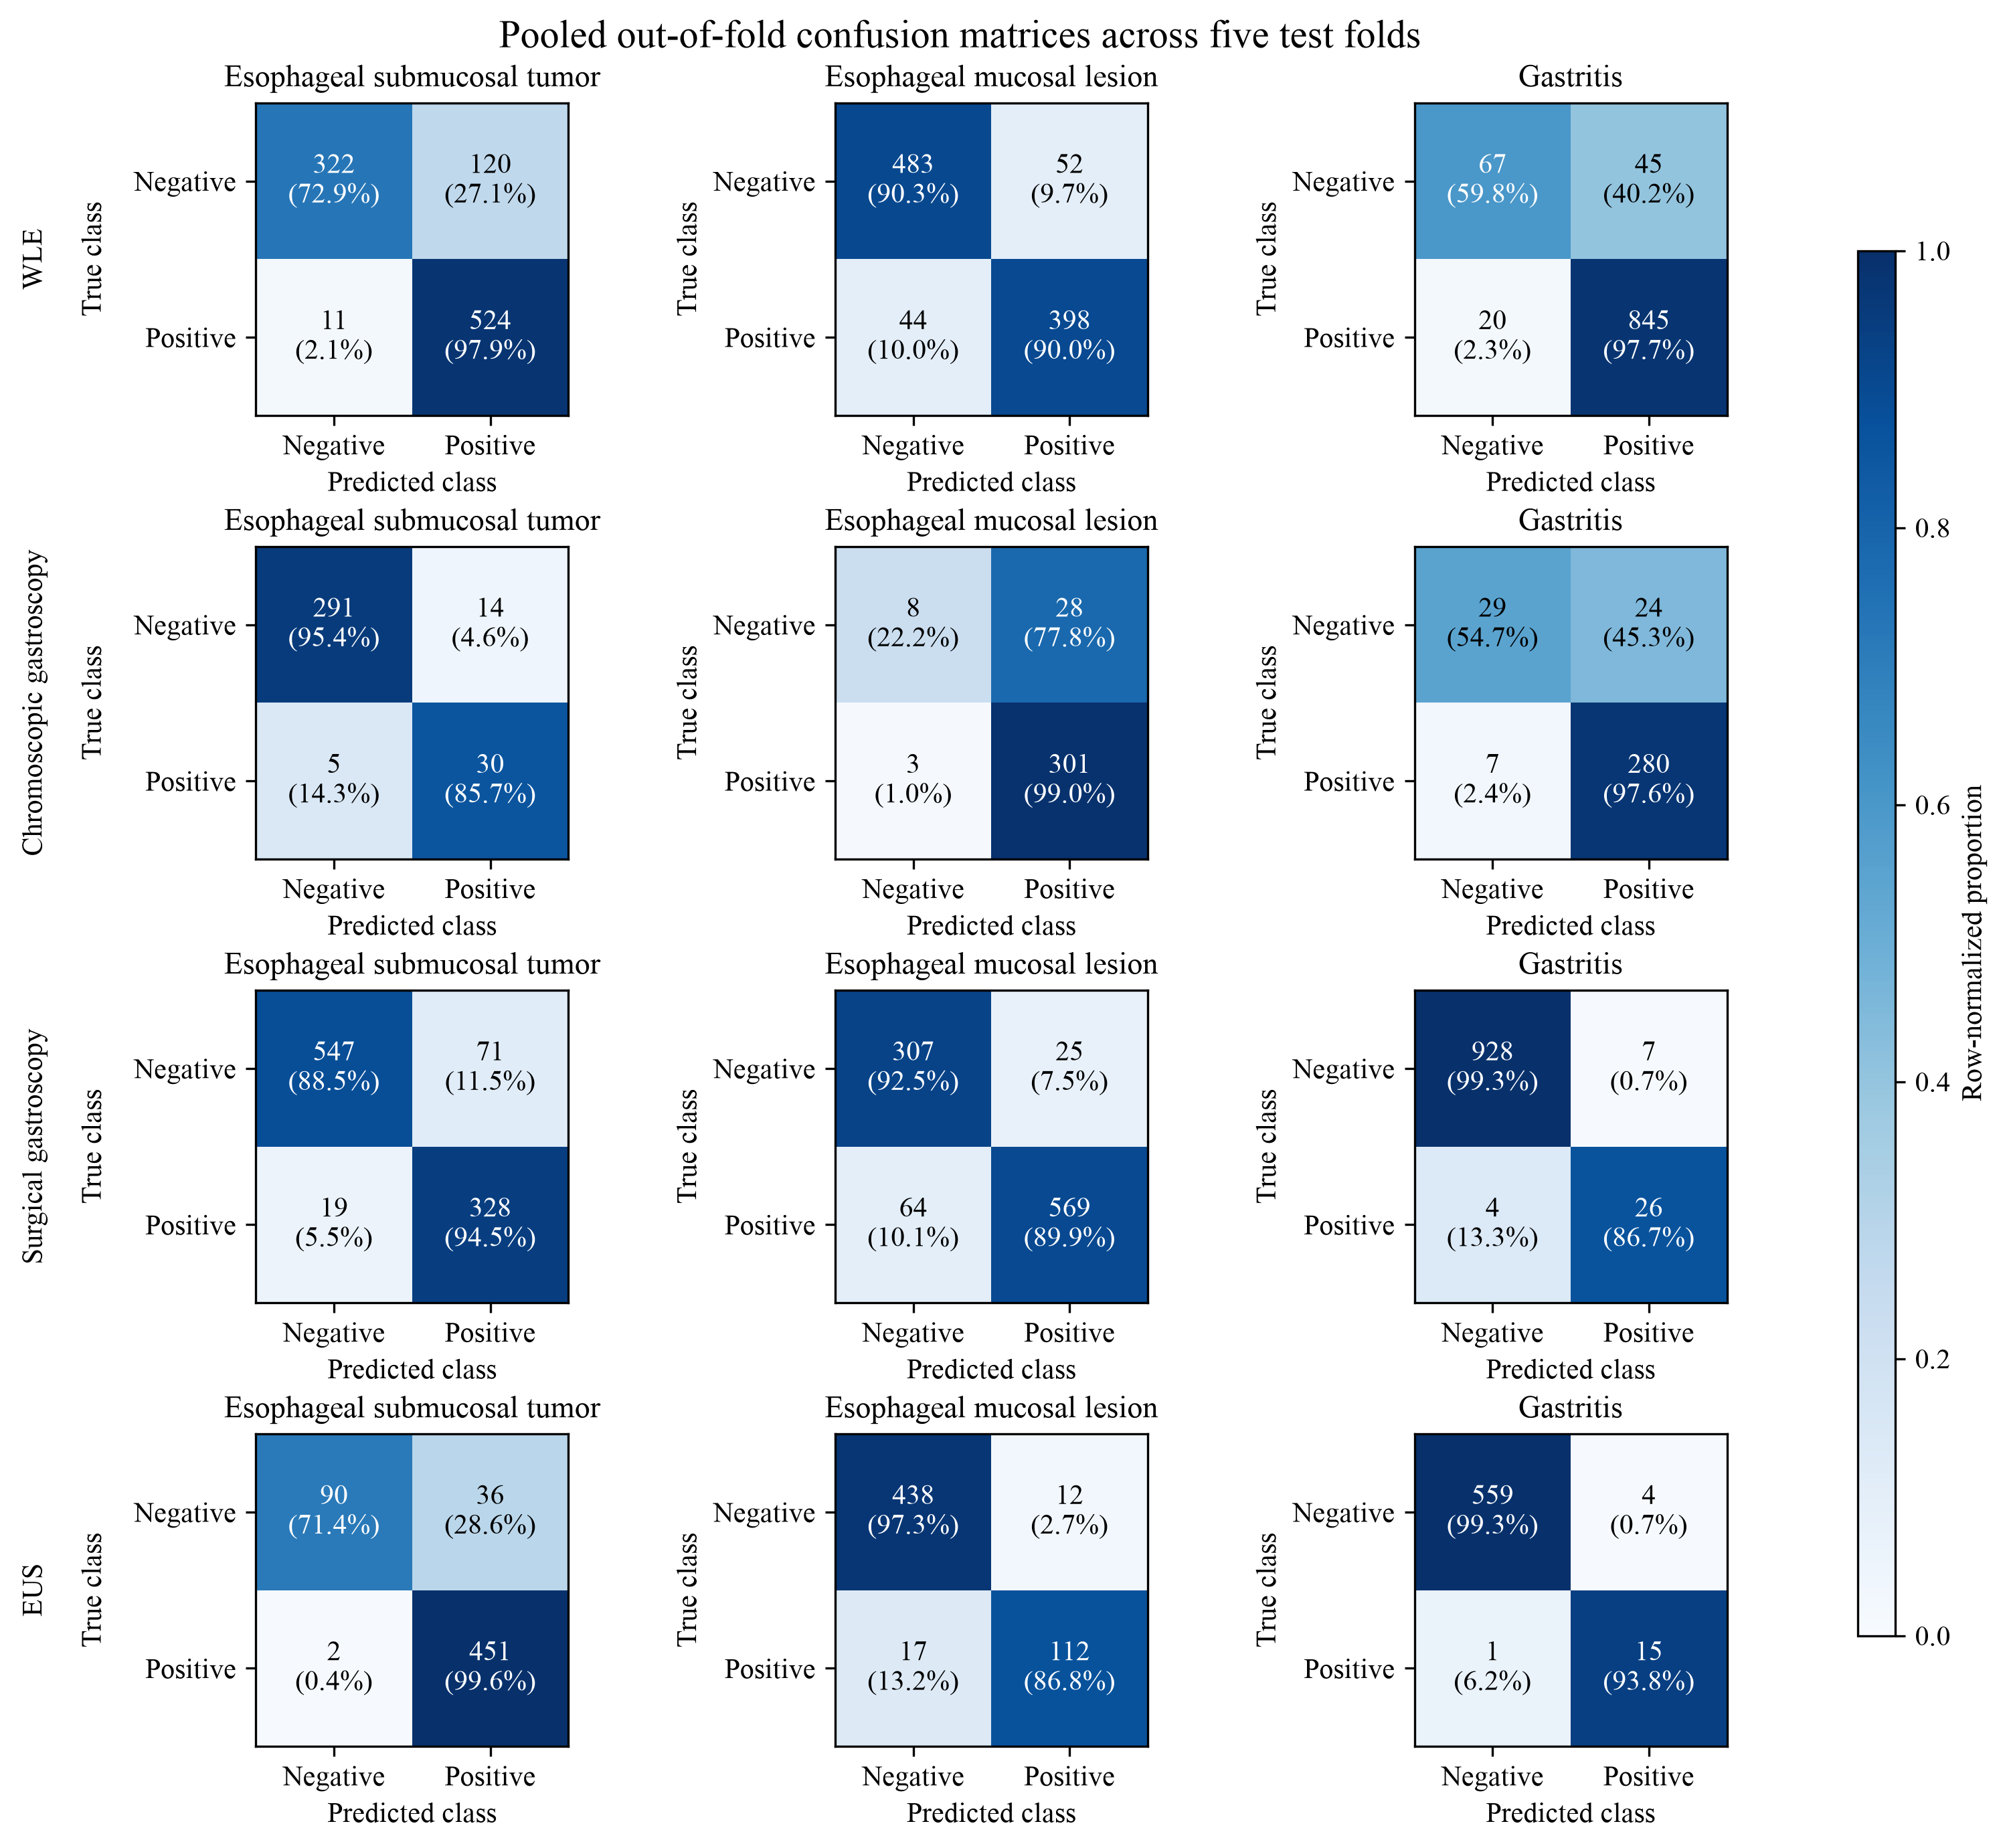
\includegraphics[width=\textwidth]{figs/selected_models_oof_confusion_matrices.png}
\caption{Pooled out-of-fold one-vs-rest confusion matrices of AMEF-MIL across the five patient-grouped test folds. Rows correspond to the WLE, chromoscopic gastroscopy, surgical gastroscopy, and EUS datasets, and columns correspond to the three target labels. Each cell reports the pooled count and the row-normalized percentage. Every examination appears in exactly one test fold.\label{fig:oof_confusion_selected}}
\end{figure*}

\subsection{Analysis and Ablation of Model Components}

\subsubsection{Image budget and position encoding}

To examine whether increasing the number of sampled images allows the model to use a larger portion of each examination effectively, we evaluated six image budgets of 16, 32, 48, 64, 80, and 96 images per examination. At every image budget, we compared the same contextual encoder without position encoding, with sampled-slot position encoding, and with APro-CoPE, thereby separating the effect of examination coverage from the effect of position modeling.

The results in Table~\ref{T3} show that increasing the image budget without position encoding produced progressively smaller gains, and the WLE performance even decreased locally at 48 and 80 images. This indicates that simply adding more images does not ensure that the contextual encoder can use the enlarged examination sequence effectively. Sampled-slot position encoding improved performance at nearly every matched budget and supported more consistent gains as additional images were introduced, particularly on chromoscopic gastroscopy, surgical gastroscopy, and EUS. APro-CoPE achieved the highest mean macro F1 in every matched dataset--budget comparison and was the only configuration whose mean performance increased monotonically from 16 to 96 images on all four datasets. The improvement was especially clear on chromoscopic gastroscopy: macro F1 increased from 0.8134 with 16 images to 0.8877 with 64 images, whereas the corresponding no-position values were 0.7478 and 0.7795. Beyond 64 images, APro-CoPE yielded only 0.16--0.52 additional percentage points across the four datasets, indicating that examination coverage approached a practical saturation point. We therefore used 64 images for the remaining ablations to retain most of the observed benefit while limiting computational cost.

\begin{table*}[t]
\scriptsize\tabletimes\centering
\caption{Effect of the sampled-image budget and position encoding across the four gastroscopy datasets. At each image budget, the same contextual encoder is evaluated without position encoding, with sampled-slot position encoding, and with APro-CoPE. Values are macro F1 reported as mean $\pm$ standard deviation over five patient-grouped folds. PE, position encoding.\label{T3}}
\resizebox{\textwidth}{!}{%
\begin{tabular}{cl*{4}{c}}
\hline
Images & Method & WLE & Chromoscopic & Surgical & EUS \\
\hline
16 & No PE & \tresult{0.8673}{0.0115} & \tresult{0.7478}{0.0513} & \tresult{0.7824}{0.0837} & \tresult{0.8443}{0.0803} \\
 & Sampled-slot PE & \tresult{0.8819}{0.0132} & \tresult{0.7789}{0.0683} & \tresult{0.8012}{0.0919} & \tresult{0.8712}{0.0663} \\
 & APro-CoPE (Ours) & \tresult{\textbf{0.8986}}{\textbf{0.0131}} & \tresult{\textbf{0.8134}}{\textbf{0.0368}} & \tresult{\textbf{0.8168}}{\textbf{0.0235}} & \tresult{\textbf{0.8879}}{\textbf{0.0635}} \\
\hline
32 & No PE & \tresult{0.8743}{0.0078} & \tresult{0.7535}{0.0341} & \tresult{0.7891}{0.0676} & \tresult{0.8537}{0.0758} \\
 & Sampled-slot PE & \tresult{0.8840}{0.0141} & \tresult{0.7978}{0.0794} & \tresult{0.8125}{0.0679} & \tresult{0.8836}{0.0749} \\
 & APro-CoPE (Ours) & \tresult{\textbf{0.9068}}{\textbf{0.0133}} & \tresult{\textbf{0.8460}}{\textbf{0.0297}} & \tresult{\textbf{0.8304}}{\textbf{0.0215}} & \tresult{\textbf{0.8979}}{\textbf{0.0564}} \\
\hline
48 & No PE & \tresult{0.8720}{0.0092} & \tresult{0.7635}{0.0438} & \tresult{0.7898}{0.0762} & \tresult{0.8594}{0.0926} \\
 & Sampled-slot PE & \tresult{0.8872}{0.0148} & \tresult{0.8249}{0.0690} & \tresult{0.8221}{0.0865} & \tresult{0.8915}{0.0672} \\
 & APro-CoPE (Ours) & \tresult{\textbf{0.9119}}{\textbf{0.0142}} & \tresult{\textbf{0.8732}}{\textbf{0.0240}} & \tresult{\textbf{0.8408}}{\textbf{0.0185}} & \tresult{\textbf{0.9030}}{\textbf{0.0434}} \\
\hline
64 & No PE & \tresult{0.8816}{0.0086} & \tresult{0.7795}{0.0351} & \tresult{0.8024}{0.0882} & \tresult{0.8694}{0.0974} \\
 & Sampled-slot PE & \tresult{0.8979}{0.0140} & \tresult{0.8592}{0.0761} & \tresult{0.8243}{0.0418} & \tresult{0.8999}{0.0617} \\
 & APro-CoPE (Ours) & \tresult{\textbf{0.9149}}{\textbf{0.0114}} & \tresult{\textbf{0.8877}}{\textbf{0.0168}} & \tresult{\textbf{0.8456}}{\textbf{0.0224}} & \tresult{\textbf{0.9064}}{\textbf{0.0474}} \\
\hline
80 & No PE & \tresult{0.8814}{0.0076} & \tresult{0.7818}{0.0426} & \tresult{0.8041}{0.0864} & \tresult{0.8715}{0.1026} \\
 & Sampled-slot PE & \tresult{0.8864}{0.0106} & \tresult{0.8665}{0.0508} & \tresult{0.8312}{0.0369} & \tresult{0.9021}{0.0598} \\
 & APro-CoPE (Ours) & \tresult{\textbf{0.9158}}{\textbf{0.0102}} & \tresult{\textbf{0.8906}}{\textbf{0.0214}} & \tresult{\textbf{0.8480}}{\textbf{0.0178}} & \tresult{\textbf{0.9089}}{\textbf{0.0452}} \\
\hline
96 & No PE & \tresult{0.8836}{0.0091} & \tresult{0.7856}{0.0397} & \tresult{0.8068}{0.0828} & \tresult{0.8731}{0.1034} \\
 & Sampled-slot PE & \tresult{0.8930}{0.0117} & \tresult{0.8706}{0.0658} & \tresult{0.8345}{0.0410} & \tresult{0.9042}{0.0635} \\
 & APro-CoPE (Ours) & \tresult{\textbf{0.9165}}{\textbf{0.0090}} & \tresult{\textbf{0.8929}}{\textbf{0.0177}} & \tresult{\textbf{0.8495}}{\textbf{0.0197}} & \tresult{\textbf{0.9103}}{\textbf{0.0442}} \\
\hline
\end{tabular}
}
\end{table*}

\subsubsection{Component analysis of APro-CoPE}

To identify which design choices contribute to APro-CoPE, we fixed the image budget at 64 and used the same two-layer bidirectional Transformer for all configurations, changing only the position mechanism. The comparison includes a Transformer without position encoding, sampled-slot position encoding, bidirectional CoPE, acquisition-anchor position encoding, and component-level variants of APro-CoPE.

The results in Table~\ref{T3_apro} show that full APro-CoPE achieved the highest mean macro F1 on all four datasets. Compared with sampled-slot position encoding, it improved macro F1 by 1.70, 2.85, 2.13, and 0.65 percentage points on WLE, chromoscopic gastroscopy, surgical gastroscopy, and EUS, respectively. Replacing the persistent transition mechanism with pairwise transitions reduced performance on all four datasets, with the largest decrease on chromoscopic gastroscopy. Removing mass conservation produced decreases of 0.28--3.25 percentage points. Retaining only the absolute route also reduced performance, whereas retaining only the relative route caused larger decreases of 0.84, 11.66, 8.10, and 7.77 percentage points. Acquisition-anchor position encoding alone did not reproduce the performance of the full method. Taken together, these comparisons show that content-adaptive transition estimation, endpoint-preserving normalization, and dual-route position delivery add complementary information to the acquisition anchor; the absolute route is particularly important for maintaining stable performance across examination settings.

\begin{table*}[t]
\footnotesize\tabletimes\centering
\caption{Component analysis of APro-CoPE across the four gastroscopy datasets using 64 sampled images per examination. All variants use the same two-layer bidirectional Transformer, and only the position mechanism is changed. Values are macro F1 reported as mean $\pm$ standard deviation over five patient-grouped folds. w/o, without; PE, position encoding; Trans., transition mechanism; CG, content gate; PW, pairwise transition used in place of PT; PT, persistent transition; AA, acquisition anchor; MC, mass conservation; Abs., absolute route; Rel., relative route.\label{T3_apro}}
\setlength{\tabcolsep}{3pt}
\resizebox{\textwidth}{!}{%
\begin{tabular}{@{}l@{\hspace{4pt}}c@{\hspace{2pt}}c@{\hspace{2pt}}c@{\hspace{2pt}}c@{\hspace{2pt}}c@{\hspace{6pt}}*{4}{c}@{}}
\hline
Position variant & Trans. & AA & MC & Abs. & Rel. & WLE & Chromoscopic & Surgical & EUS \\
\hline
Transformer w/o PE & -- & -- & -- & -- & -- & \tresult{0.8816}{0.0086} & \tresult{0.7795}{0.0351} & \tresult{0.8024}{0.0882} & \tresult{0.8694}{0.0974} \\
Sampled-slot PE & -- & -- & -- & $\checkmark$ & -- & \tresult{0.8979}{0.0140} & \tresult{0.8592}{0.0761} & \tresult{0.8243}{0.0418} & \tresult{0.8999}{0.0617} \\
Bidirectional CoPE & CG & -- & -- & -- & $\checkmark$ & \tresult{0.9067}{0.0059} & \tresult{0.7535}{0.0357} & \tresult{0.7891}{0.1004} & \tresult{0.8537}{0.0996} \\
Acquisition-anchor PE & -- & $\checkmark$ & -- & $\checkmark$ & -- & \tresult{0.9105}{0.0039} & \tresult{0.8592}{0.0586} & \tresult{0.8112}{0.0736} & \tresult{0.8999}{0.0731} \\
APro-CoPE w/o Trans. & PW & $\checkmark$ & $\checkmark$ & $\checkmark$ & $\checkmark$ & \tresult{0.9102}{0.0070} & \tresult{0.8391}{0.0759} & \tresult{0.8356}{0.0807} & \tresult{0.8900}{0.0572} \\
APro-CoPE w/o MC & PT & $\checkmark$ & -- & $\checkmark$ & $\checkmark$ & \tresult{0.9121}{0.0118} & \tresult{0.8552}{0.0187} & \tresult{0.8131}{0.0625} & \tresult{0.8974}{0.0760} \\
APro-CoPE w/o Rel. & PT & $\checkmark$ & $\checkmark$ & $\checkmark$ & -- & \tresult{0.9101}{0.0057} & \tresult{0.8274}{0.0811} & \tresult{0.8289}{0.0681} & \tresult{0.8957}{0.0658} \\
APro-CoPE w/o Abs. & PT & $\checkmark$ & $\checkmark$ & -- & $\checkmark$ & \tresult{0.9065}{0.0086} & \tresult{0.7711}{0.0557} & \tresult{0.7646}{0.1039} & \tresult{0.8287}{0.0879} \\
Full APro-CoPE (Ours) & PT & $\checkmark$ & $\checkmark$ & $\checkmark$ & $\checkmark$ & \tresult{\textbf{0.9149}}{\textbf{0.0114}} & \tresult{\textbf{0.8877}}{\textbf{0.0168}} & \tresult{\textbf{0.8456}}{\textbf{0.0224}} & \tresult{\textbf{0.9064}}{\textbf{0.0474}} \\
\hline
\end{tabular}
}
\end{table*}

\subsubsection{Qualitative analysis of APro-CoPE under subsampling and full-sequence retention}

To qualitatively illustrate how APro-CoPE constructs acquisition-anchored, content-adaptive position relationships for both subsampled and fully retained examination sequences, we visualized representative cases under a maximum image budget of $T=64$. An examination containing more than 64 images was represented by 64 uniformly subsampled images, with their original acquisition order and indices preserved; an examination containing at most 64 images retained its full image sequence. Figure~\ref{fig:apro_cope_length_groups} presents both input-construction settings using examples from the four gastroscopy datasets. For each example, the image strip presents the sequence supplied to the model, the orange curve measures the feature change between adjacent images, the blue dashed curve measures the relative interval change from original acquisition positions to uniformly spaced sampled slots, and the red curve measures the relative interval change from acquisition anchors to the contextual coordinates produced by APro-CoPE. The blue curve therefore characterizes the position change introduced during input construction, while the red curve characterizes the subsequent content-adaptive adjustment.

\begin{figure*}[t]
\centering
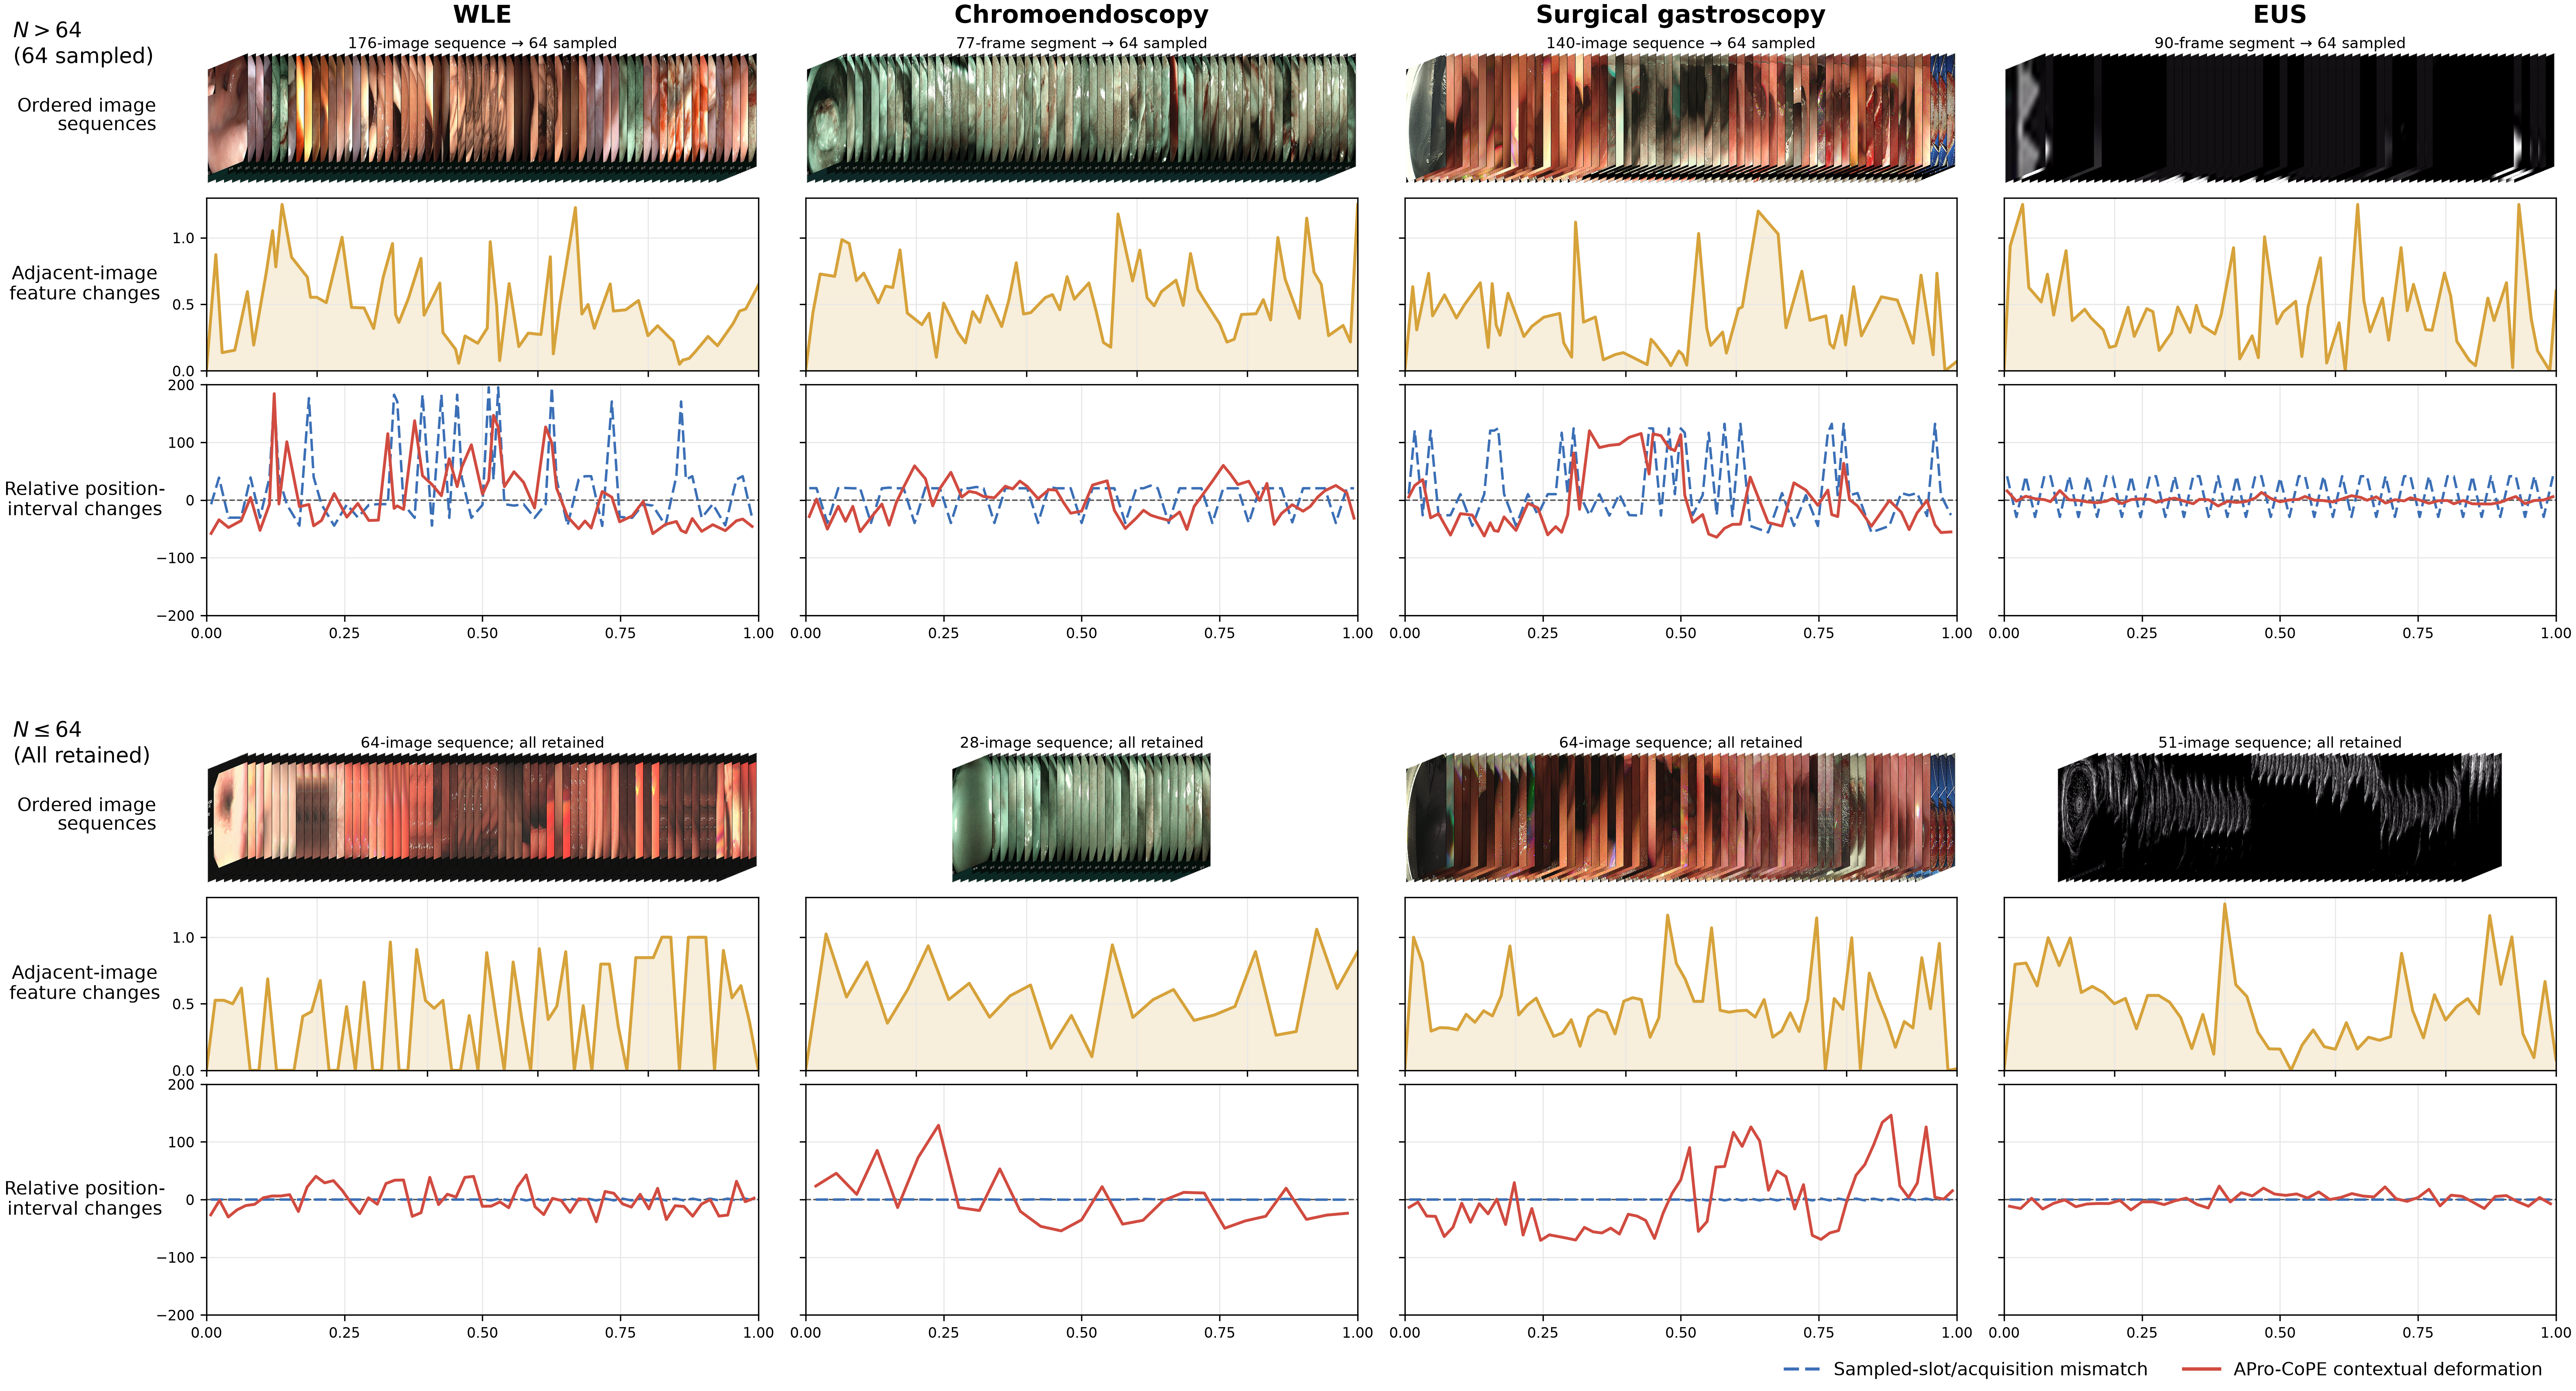
\includegraphics[width=\textwidth]{figs/apro_cope_mechanism_length_groups_four_datasets.png}
\caption{Qualitative visualization of APro-CoPE under subsampling and full-sequence retention. With a maximum image budget of $T=64$, the upper group uniformly subsamples 64 images when $N>64$, and the lower group retains the full sequence when $N\leq64$.\label{fig:apro_cope_length_groups}}
\end{figure*}

Uniform subsampling produced visible blue fluctuations because the selected images retained their positions within the complete acquisition sequence, whereas full-sequence retention yielded blue values close to zero through direct correspondence between image order and sampled slots. Against these acquisition anchors, the red curves formed distinct patterns for individual examinations under both input-construction settings, showing how APro-CoPE redistributed contextual intervals according to image content. The red deformation patterns followed the continuity of visual changes across neighboring images, reflecting content-adaptive interval adjustment driven by persistent image transitions. Particularly in the EUS examples, several isolated peaks in adjacent-image feature change coincided with relatively small overall red adjustments; by comparison, the WLE, chromoendoscopy, and surgical gastroscopy examples showed stronger adjustments within sequence segments containing sustained visual changes. Together, these patterns illustrate examination-specific position modeling for both subsampled and fully retained inputs.

\subsubsection{Effect of APro-CoPE on examination-level prediction quality}

Figure~\ref{fig:apro_cope_prediction_distributions} compares the examination-level distributions of label-wise accuracy, true-class confidence, and Brier score between sampled-slot PE and full APro-CoPE under the 64-image setting. Label-wise accuracy is the proportion of the three binary labels classified correctly. True-class confidence is the mean probability assigned to the correct binary outcome, and the Brier score is the mean squared difference between the predicted probabilities and binary targets. Therefore, higher label-wise accuracy indicates more correct label decisions, higher true-class confidence indicates greater confidence in the correct outcomes, and a lower Brier score indicates smaller probability error; together, these values indicate better examination-level prediction quality.

Compared with sampled-slot PE, APro-CoPE achieved higher mean label-wise accuracy on WLE, chromoscopic gastroscopy, and EUS; only surgical gastroscopy showed a small decrease, from 0.9179 to 0.9160. Mean true-class confidence was also higher on WLE, chromoscopic gastroscopy, and surgical gastroscopy; only EUS showed a small decrease, from 0.9079 to 0.9025. The mean Brier score was lower with APro-CoPE on all four datasets. The largest reduction occurred on chromoscopic gastroscopy, from 0.0809 to 0.0730, followed by EUS, from 0.0463 to 0.0403. Thus, APro-CoPE improved label correctness and confidence in the correct outcomes on most datasets and reduced probability error on all four datasets, indicating an overall improvement in examination-level prediction quality. These distributional improvements also help explain the more pronounced advantage of APro-CoPE over sampled-slot PE on chromoscopic gastroscopy in the preceding experiments.

\begin{figure*}[t]
\centering
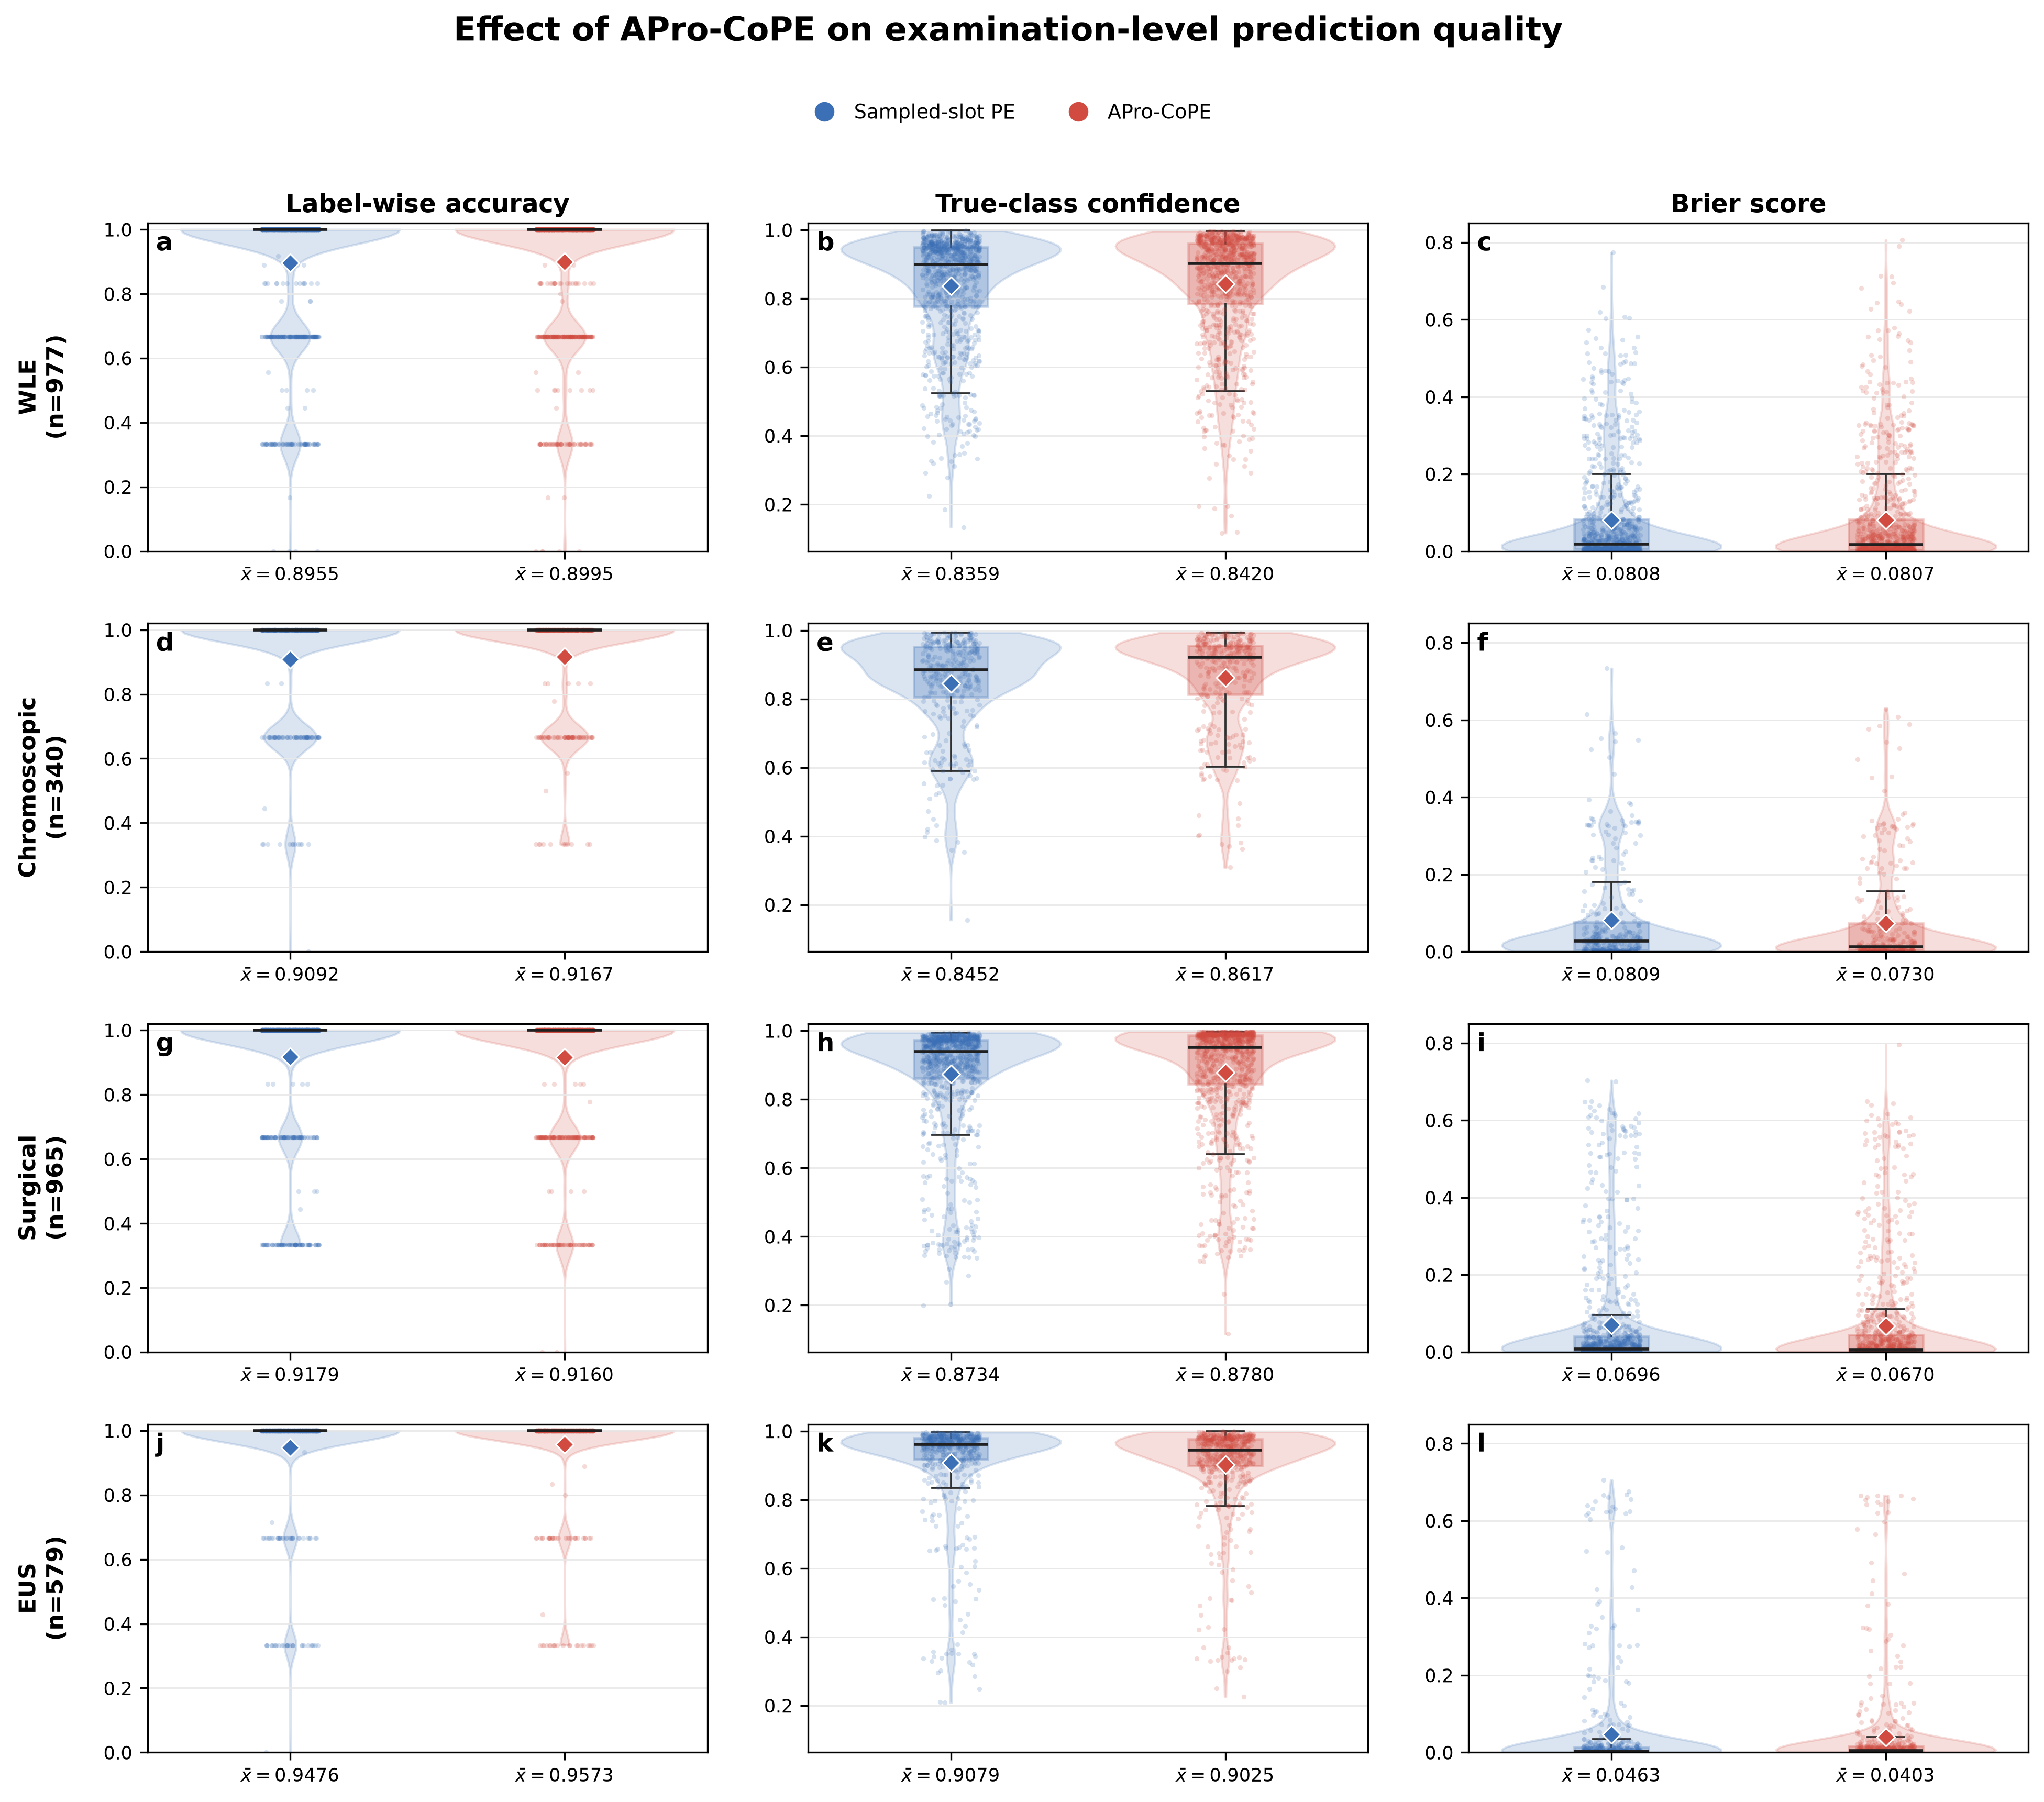
\includegraphics[width=\textwidth]{figs/apro_cope_examination_level_prediction_distributions.png}
\caption{Effect of APro-CoPE on examination-level prediction quality relative to sampled-slot position encoding across the four gastroscopy datasets. Rows correspond to WLE, chromoscopic gastroscopy, surgical gastroscopy, and EUS; columns show label-wise accuracy, true-class confidence, and Brier score. Each point represents one examination evaluated in its held-out test fold. For examinations with more than 64 images, metrics were averaged over acquisition-ordered stratified samples covering the original sequence, with at most five sampling passes. Violin shapes show the distributions, boxes show the interquartile ranges and medians, diamonds show the arithmetic means, and $\bar{x}$ reports the corresponding mean values. Higher label-wise accuracy and true-class confidence are preferable, whereas a lower Brier score is preferable.\label{fig:apro_cope_prediction_distributions}}
\end{figure*}

\subsubsection{Ablation of multi-label attention MIL and label hypergraph reasoning}

To distinguish the contributions of label-specific image aggregation and higher-order label reasoning, we conducted the targeted ablation summarized in Table~\ref{T_label_reasoning}. Starting from shared-attention MIL without label reasoning, we introduced multi-label attention MIL and then compared no label reasoning, an ordinary learnable label graph, and the proposed label hypergraph.

Replacing shared-attention MIL with multi-label attention MIL consistently improved macro F1 by 0.56--0.61 percentage points across the four datasets. Adding the ordinary label graph produced further gains of 0.56--0.62 percentage points, while replacing it with the label hypergraph yielded larger additional gains of 1.86--3.59 percentage points. The model configuration combining multi-label attention with label hypergraph reasoning achieved the highest macro F1 on every dataset and improved over the shared-attention baseline by 3.09--4.76 percentage points, supporting the complementary roles of label-specific image aggregation and higher-order label reasoning.

\begin{table*}[t]
\scriptsize\tabletimes\centering
\caption{Targeted ablation of multi-label attention MIL and label hypergraph reasoning across the four gastroscopy datasets using 64 sampled images per examination. Acquisition-aware visual context modeling, label-query cross-attention, and gated residual fusion were retained in all configurations. Values are macro F1 reported as mean $\pm$ standard deviation over five patient-grouped folds.\label{T_label_reasoning}}
\resizebox{\textwidth}{!}{%
\begin{tabular}{ll*{4}{c}}
\hline
MIL aggregation & Label reasoner & WLE & Chromoscopic & Surgical & EUS \\
\hline
Shared attention & -- & \tresult{0.8840}{0.0148} & \tresult{0.8401}{0.0465} & \tresult{0.8054}{0.0479} & \tresult{0.8732}{0.0691} \\
Multi-label attention & -- & \tresult{0.8901}{0.0141} & \tresult{0.8460}{0.0438} & \tresult{0.8110}{0.0447} & \tresult{0.8792}{0.0658} \\
Multi-label attention & Label graph & \tresult{0.8963}{0.0135} & \tresult{0.8518}{0.0406} & \tresult{0.8166}{0.0408} & \tresult{0.8853}{0.0623} \\
Multi-label attention & Label hypergraph & \tresult{\textbf{0.9149}}{\textbf{0.0114}} & \tresult{\textbf{0.8877}}{\textbf{0.0168}} & \tresult{\textbf{0.8456}}{\textbf{0.0224}} & \tresult{\textbf{0.9064}}{\textbf{0.0474}} \\
\hline
\end{tabular}
}
\par\raggedright\scriptsize MIL, multiple instance learning; Label graph denotes an ordinary learnable label graph.
\end{table*}

To determine whether the performance gains in Table~\ref{T_label_reasoning} were accompanied by label-specific visual evidence allocation, we compared the overlap among label-wise image-evidence sets across the four gastroscopy datasets (Figure~\ref{fig:label_evidence_overlap}). Our model's multi-label attention module consistently remained among the methods with the strongest evidence separation, showing that it assigned differentiated supporting images to individual diseases across examination settings. This result provides a basis for further assessing whether the differentiated evidence contributes selectively to the corresponding label decisions.

\begin{figure*}[t]
\centering
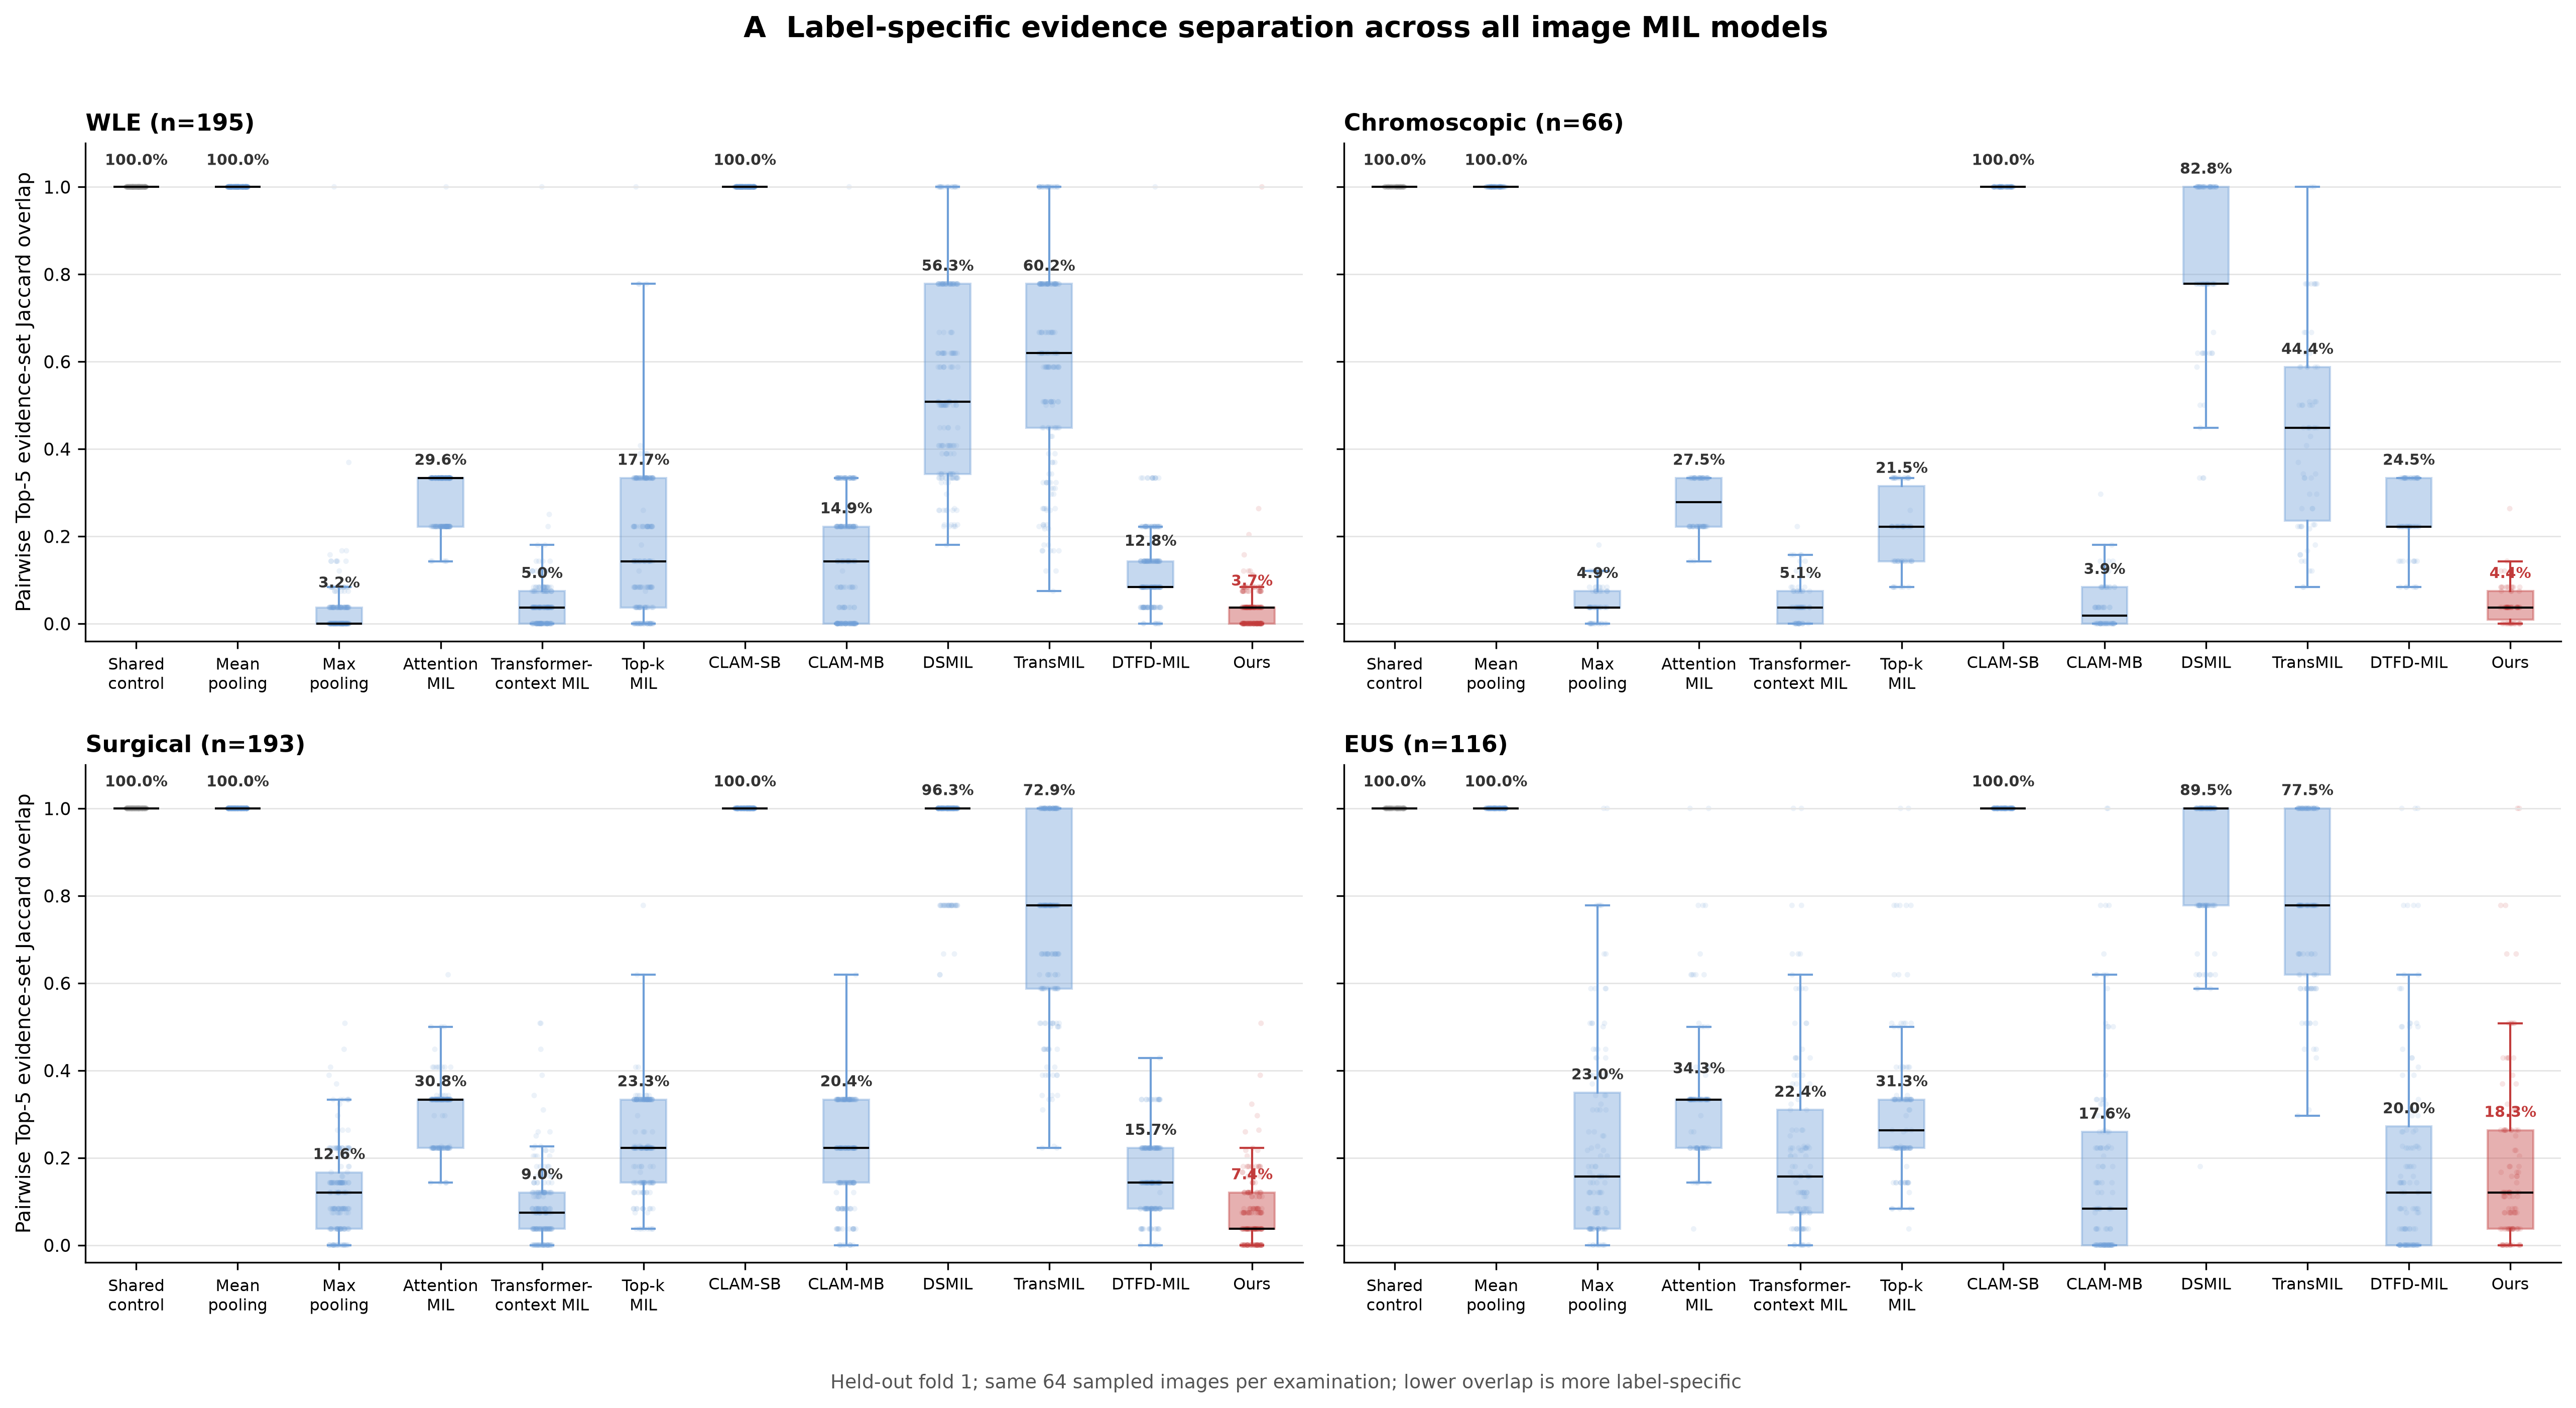
\includegraphics[width=\textwidth]{figs/label_specific_evidence_overlap_four_datasets.png}
\caption{Label-specific image-evidence separation across the compared MIL architectures. For each held-out fold-1 examination, the same set of up to 64 uniformly sampled images was ranked separately for each of the three labels, and the mean pairwise Jaccard overlap among their Top-5 evidence sets was calculated. Each point represents one examination, boxes show the interquartile ranges and medians, and percentages report arithmetic means. Lower overlap indicates stronger separation of label-specific supporting evidence.\label{fig:label_evidence_overlap}}
\end{figure*}

To further assess whether the separated evidence contributed selectively to the corresponding label decisions, we performed label-targeted deletion (Figure~\ref{fig:label_targeted_deletion}). Compared with the shared-attention control, our model's multi-label attention module exhibited stronger diagonal concentration in most examination settings. After removing the high-attention evidence associated with a given label, the resulting decision impact was concentrated more strongly on that label's own prediction, indicating that the module learned label-specific visual evidence. Taken together, the lower cross-label evidence overlap and stronger label-specific decision impact indicate that evidence separation and label-specific decision-making reduce evidence interference across labels, thereby contributing to the higher macro F1 achieved by the model configuration combining multi-label attention with label hypergraph reasoning.

\begin{figure*}[t]
\centering
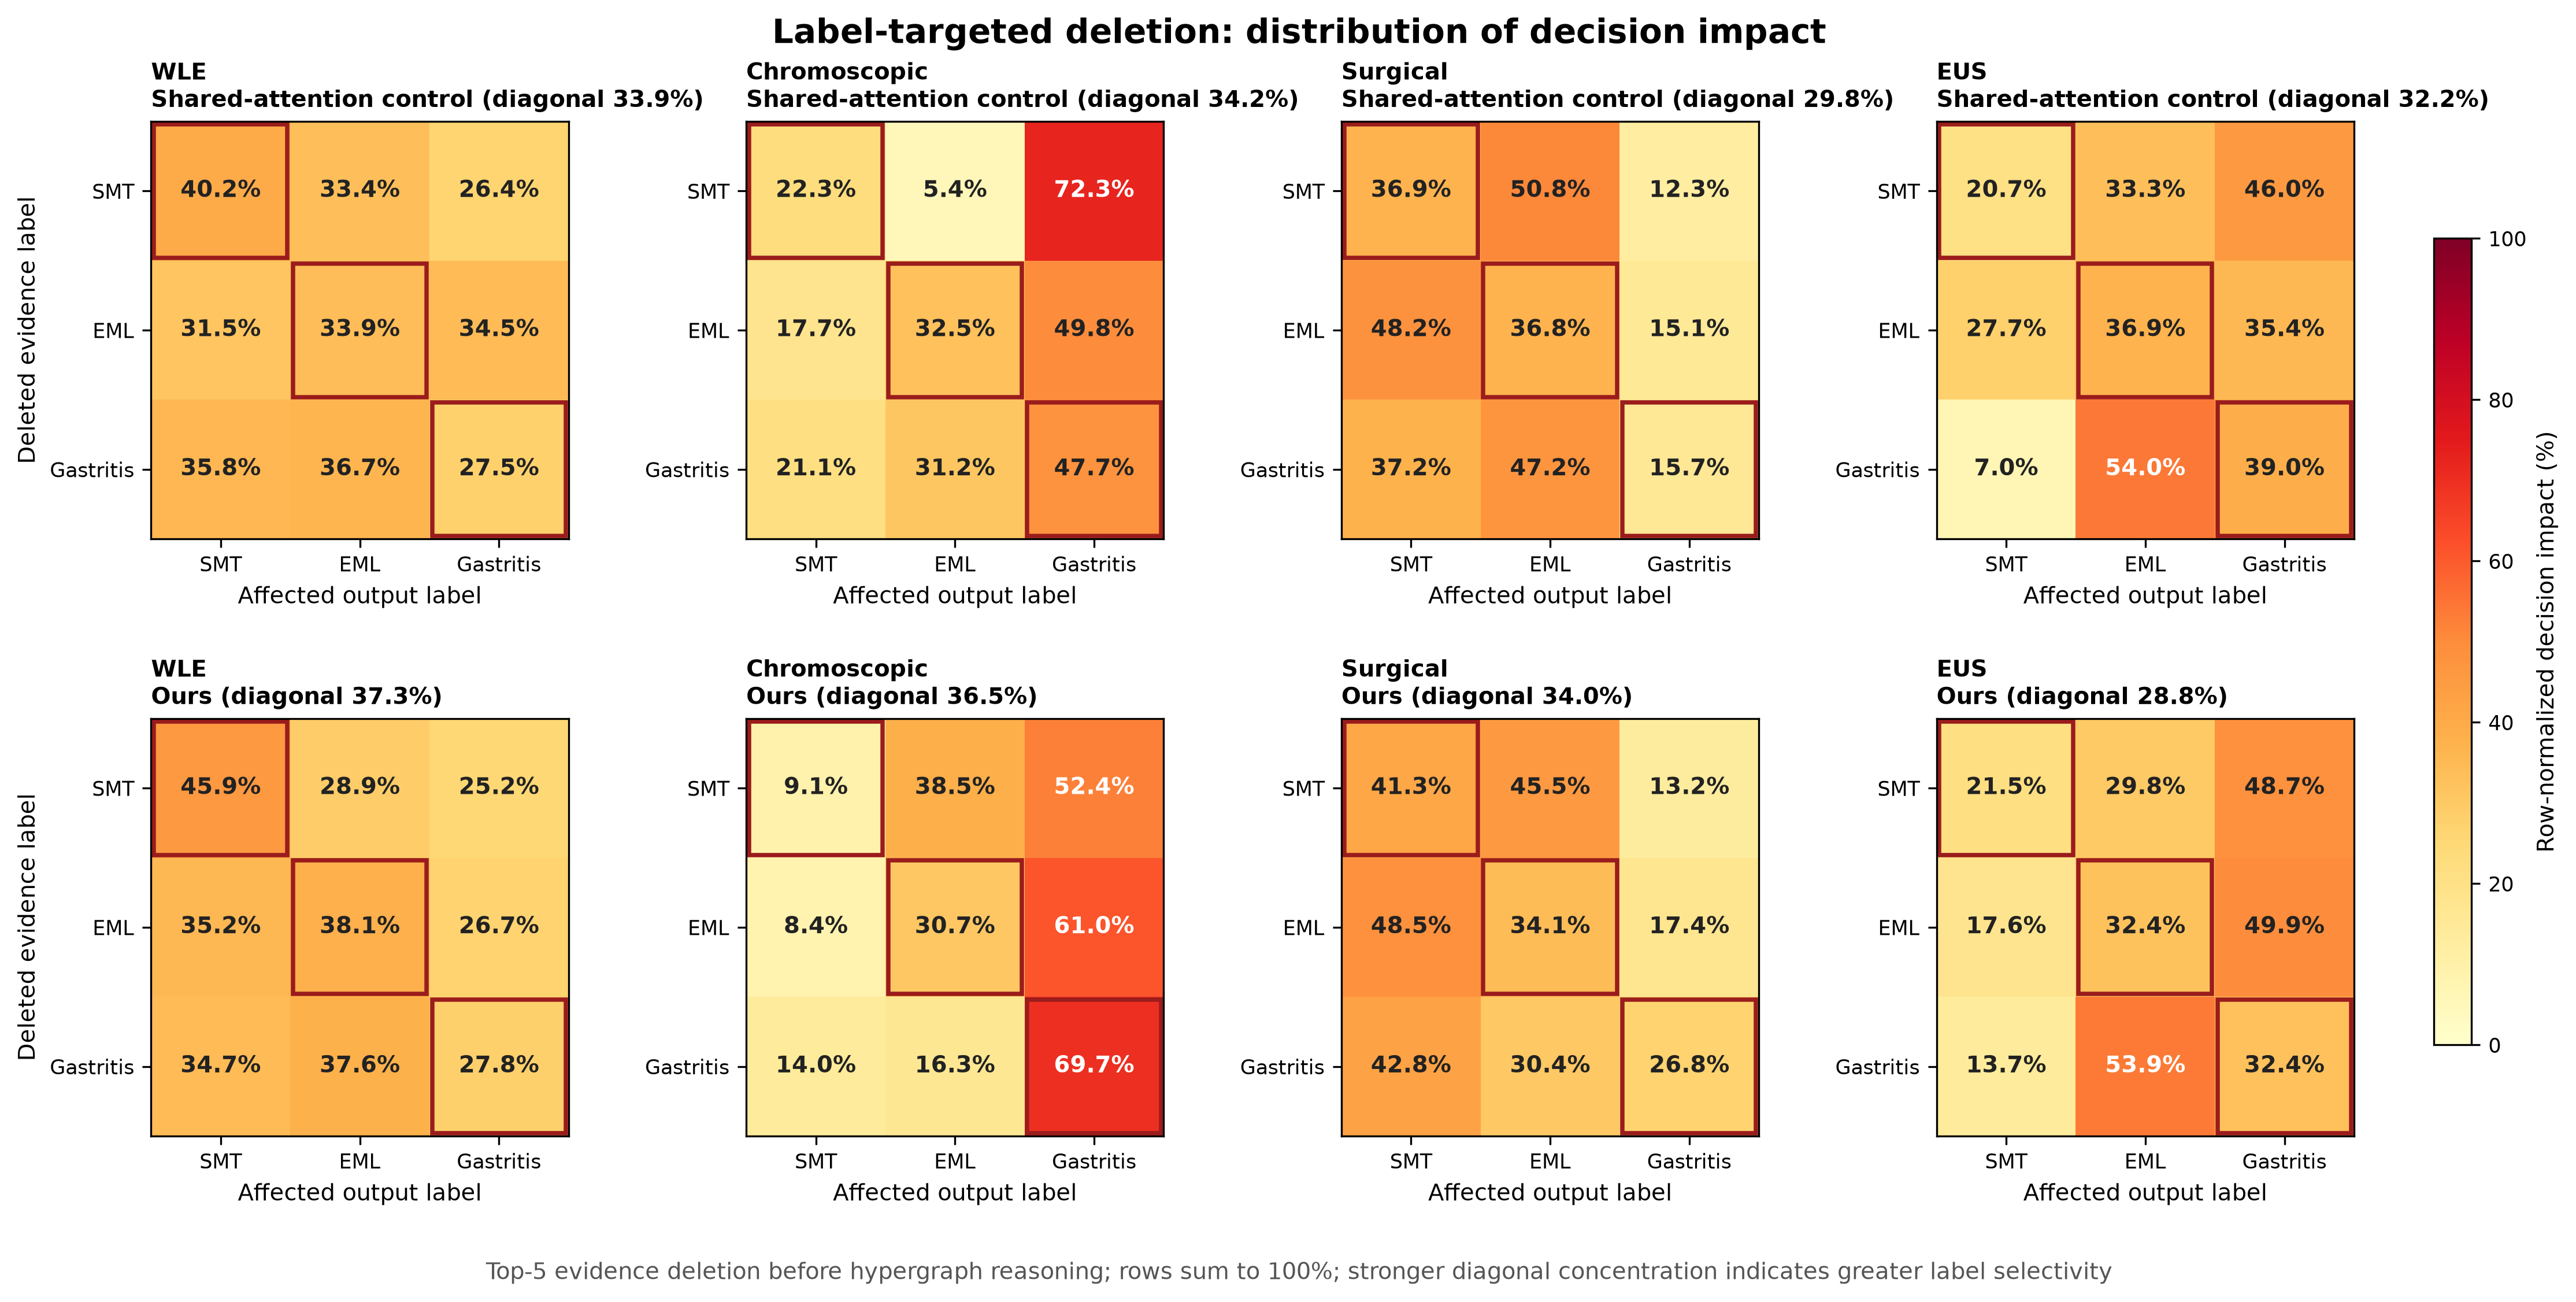
\includegraphics[width=\textwidth]{figs/label_targeted_deletion_selectivity_four_datasets.png}
\caption{Label-targeted deletion analysis across the four gastroscopy datasets. For each deleted-evidence label (rows), its Top-5 attended images were removed before label hypergraph reasoning, and the resulting decision impact was distributed across the three output labels (columns) and normalized to sum to 100\% within each row. The upper panels show the shared-attention control, and the lower panels show the proposed model. Red outlines mark matching deleted and affected labels; stronger diagonal concentration indicates greater label-specific decision selectivity.\label{fig:label_targeted_deletion}}
\end{figure*}

To examine the contribution of label hypergraph reasoning more directly in examinations containing coexisting findings, we further stratified positive labels according to whether an examination contained a single positive target or multiple co-positive targets (Figure~\ref{fig:label_hypergraph_copositive_confidence}). The single-positive group was retained as a reference. In this group, the label hypergraph yielded slightly lower confidence than the ordinary label graph in some datasets, which is consistent with its design focus on higher-order relationships among coexisting diseases rather than isolated positive labels. In contrast, in the co-positive group, label hypergraph reasoning achieved the highest mean positive-label confidence across all four datasets, consistently exceeding both no label reasoning and the ordinary label graph. This pattern indicates that higher-order label interactions strengthen the integration of evidence for coexisting diseases, thereby contributing to the higher macro F1 achieved by the model configuration combining multi-label attention with label hypergraph reasoning in Table~\ref{T_label_reasoning}.

\begin{figure*}[t]
\centering
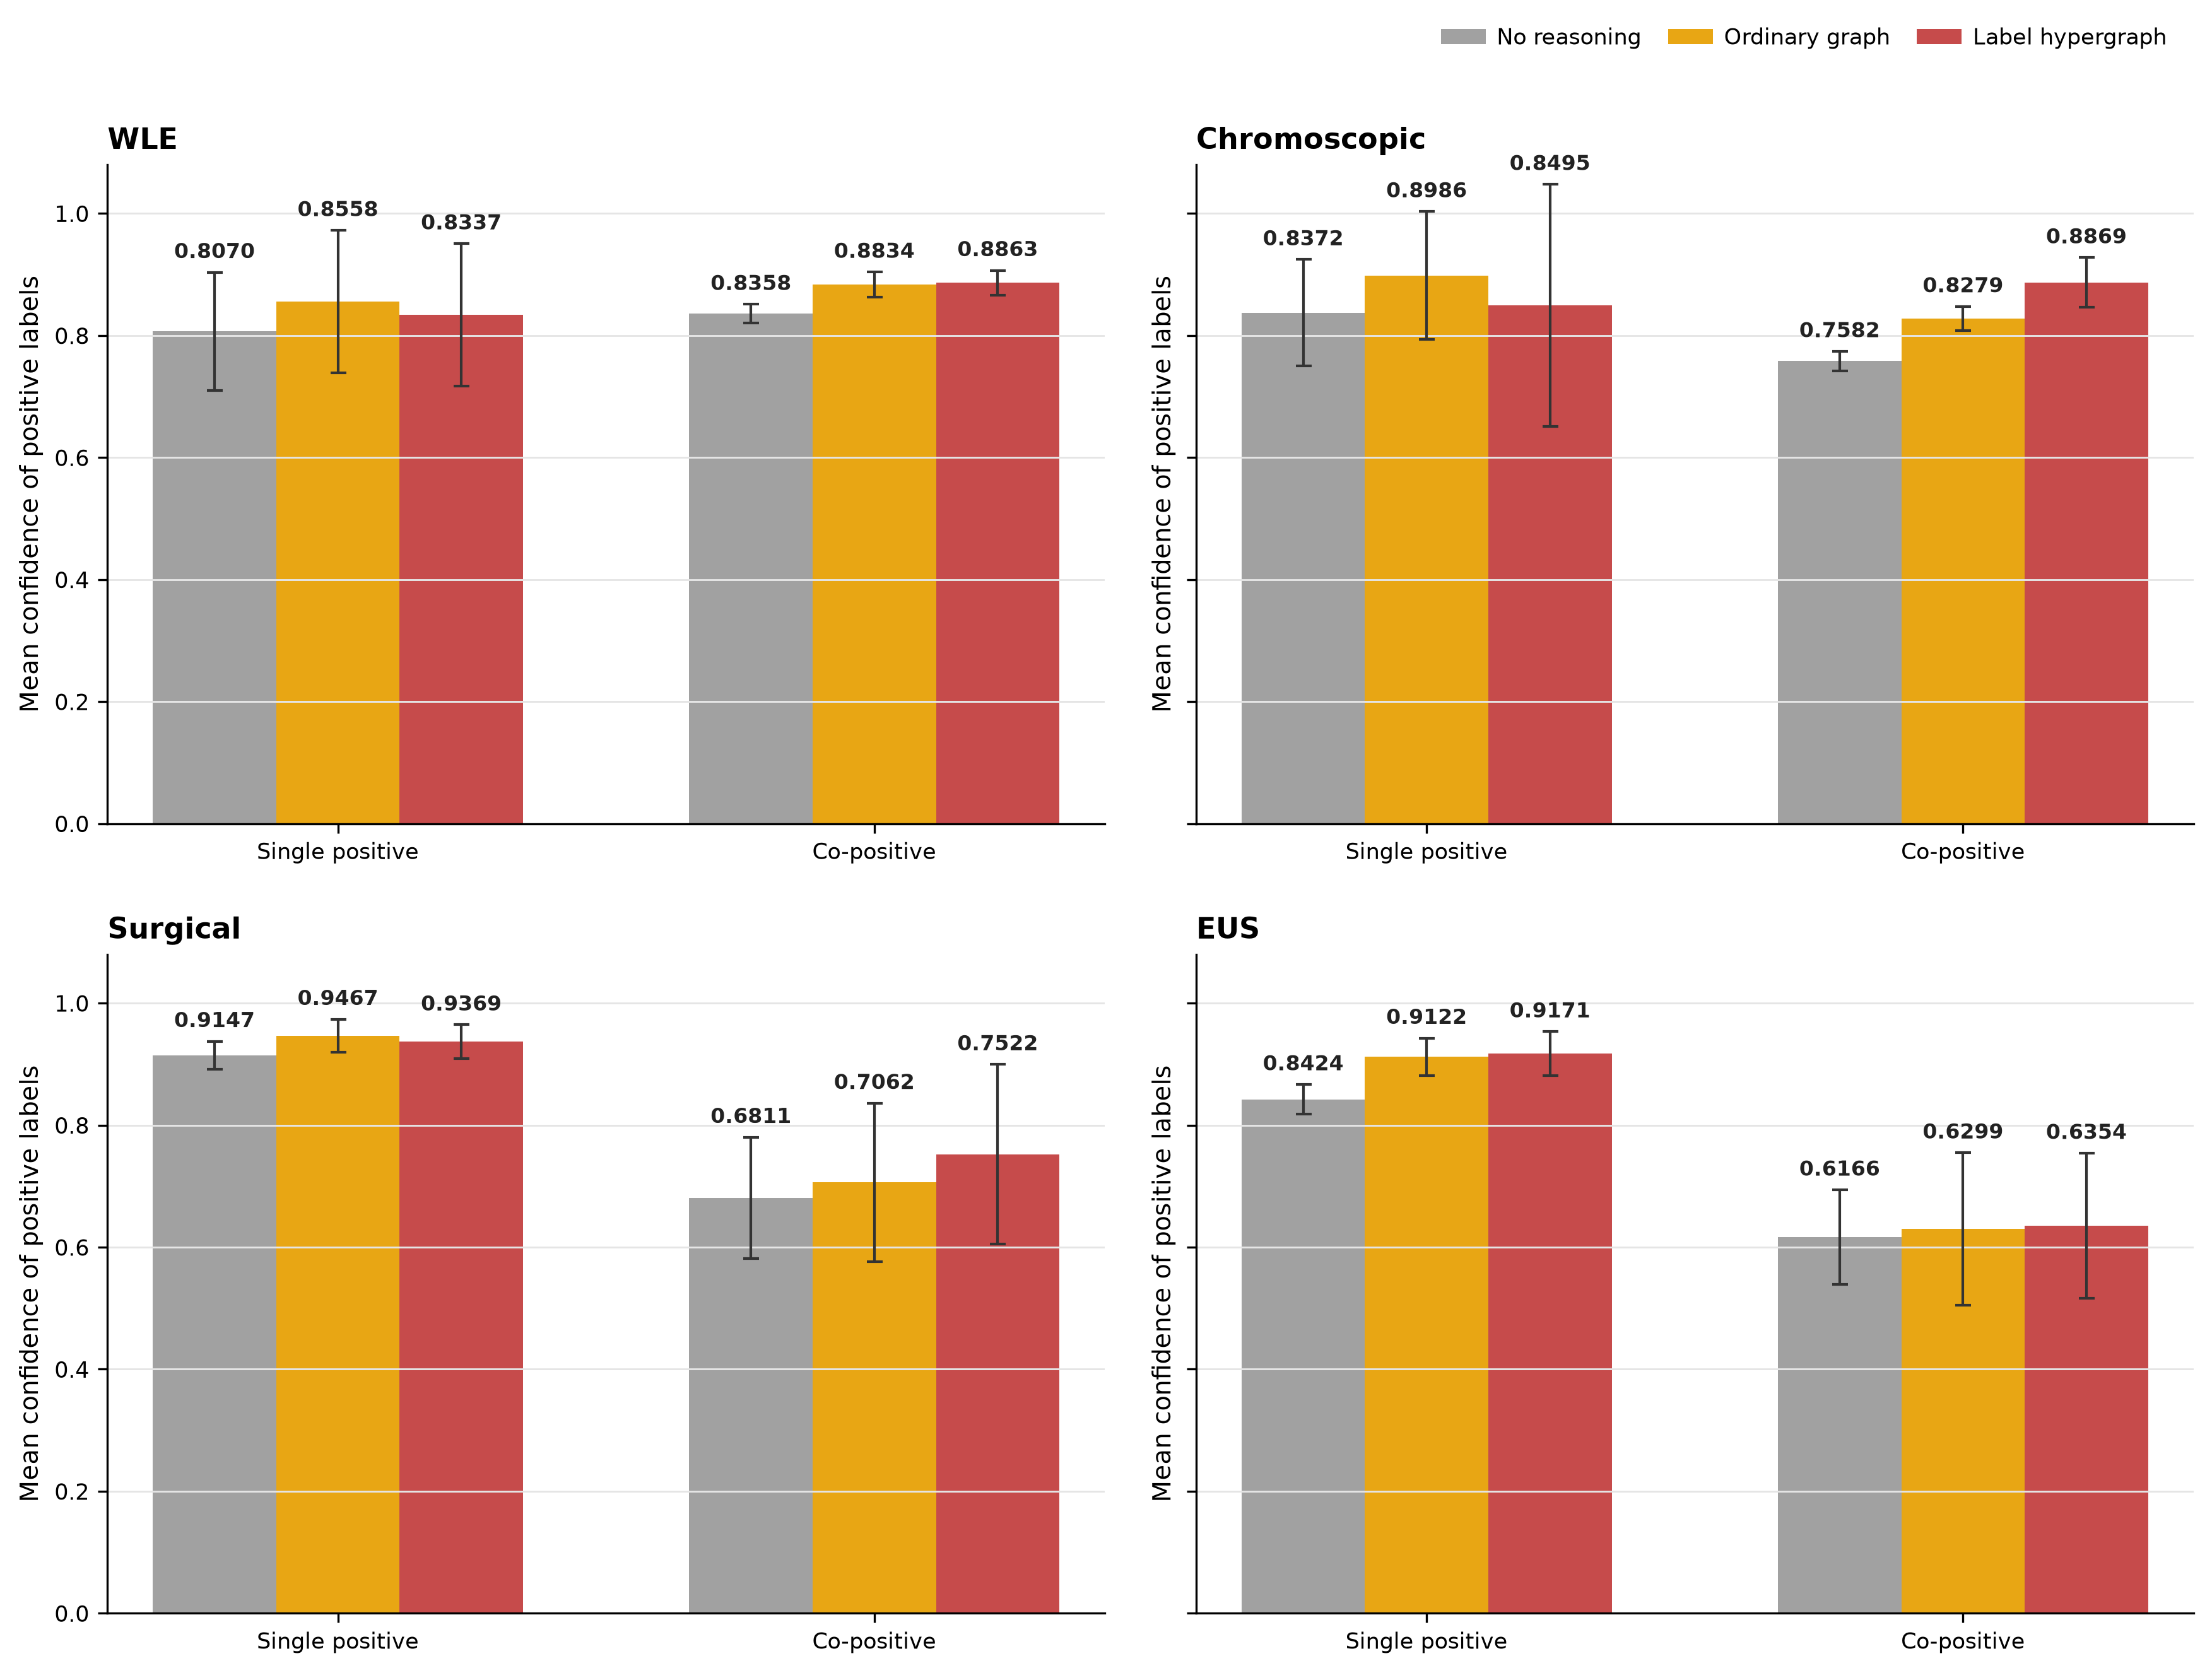
\includegraphics[width=\textwidth]{figs/label_hypergraph_copositive_confidence_four_datasets.png}
\caption{Positive-label confidence under different label-set complexities across the four gastroscopy datasets. Examinations were divided into single-positive and co-positive groups according to the number of positive target labels. Bars show the mean confidence assigned to positive labels, and error bars indicate 95\% confidence intervals. The compared configurations used multi-label attention and differed in their label-reasoning mechanism.\label{fig:label_hypergraph_copositive_confidence}}
\end{figure*}

\subsubsection{Ablation of label-conditioned cross-modal retrieval and adaptive residual fusion}

To disentangle the individual and joint contributions of label-conditioned textual retrieval and adaptive residual fusion, we conducted a targeted $2\times2$ ablation of label-query cross-attention (LQCA) and gated residual fusion (GRF). The experiment compared a baseline without either component with configurations enabling LQCA alone, GRF alone, or both components. The results are summarized in Table~\ref{T_crossmodal_fusion}.

Label-query retrieval and gated fusion each improved over the visual pathway, while their combination achieved the highest macro F1 on every dataset, with gains of 2.42--4.40 percentage points. These results support the complementary roles of label-conditioned retrieval and adaptive control of the retrieved textual evidence.

\begin{table*}[t]
\scriptsize\tabletimes\centering
\caption{$2\times2$ ablation of label-query cross-attention and gated residual fusion across the four gastroscopy datasets using 64 sampled images per examination. APro-CoPE-based acquisition-aware context modeling and label hypergraph reasoning were retained in all configurations. Values are macro F1 reported as mean $\pm$ standard deviation over five patient-grouped folds.\label{T_crossmodal_fusion}}
\resizebox{\textwidth}{!}{%
\begin{tabular}{cc*{4}{c}}
\hline
Text retrieval & Residual fusion & WLE & Chromoscopic & Surgical & EUS \\
\hline
-- & -- & \tresult{0.8907}{0.0110} & \tresult{0.8437}{0.0524} & \tresult{0.8055}{0.0600} & \tresult{0.8769}{0.0675} \\
LQCA & -- & \tresult{0.9031}{0.0128} & \tresult{0.8658}{0.0320} & \tresult{0.8267}{0.0456} & \tresult{0.8921}{0.0567} \\
-- & GRF & \tresult{0.9056}{0.0119} & \tresult{0.8693}{0.0437} & \tresult{0.8299}{0.0491} & \tresult{0.8940}{0.0538} \\
LQCA & GRF & \tresult{\textbf{0.9149}}{\textbf{0.0114}} & \tresult{\textbf{0.8877}}{\textbf{0.0168}} & \tresult{\textbf{0.8456}}{\textbf{0.0224}} & \tresult{\textbf{0.9064}}{\textbf{0.0474}} \\
\hline
\end{tabular}
}
\par\raggedright\scriptsize LQCA, label-query cross-attention; GRF, gated residual fusion.
\end{table*}

To further determine whether the improvement associated with LQCA reflected label-specific textual retrieval, we compared positive-label confidence under three retrieval conditions across the four gastroscopy datasets (Figure~\ref{fig:label_query_retrieval_specificity}). The correct condition retained the text representation retrieved by the corresponding label query, the cross-label condition reassigned retrieved representations across labels, and the pooled condition used a shared description representation. Positive-label confidence was highest under the correct label-query correspondence and decreased after cross-label reassignment or shared pooling. This pattern indicates that disease-matched label queries retrieve more effective label-specific textual evidence, thereby supporting the macro F1 improvement obtained by the model configuration using label-query cross-attention in Table~\ref{T_crossmodal_fusion}.

\begin{figure*}[t]
\centering
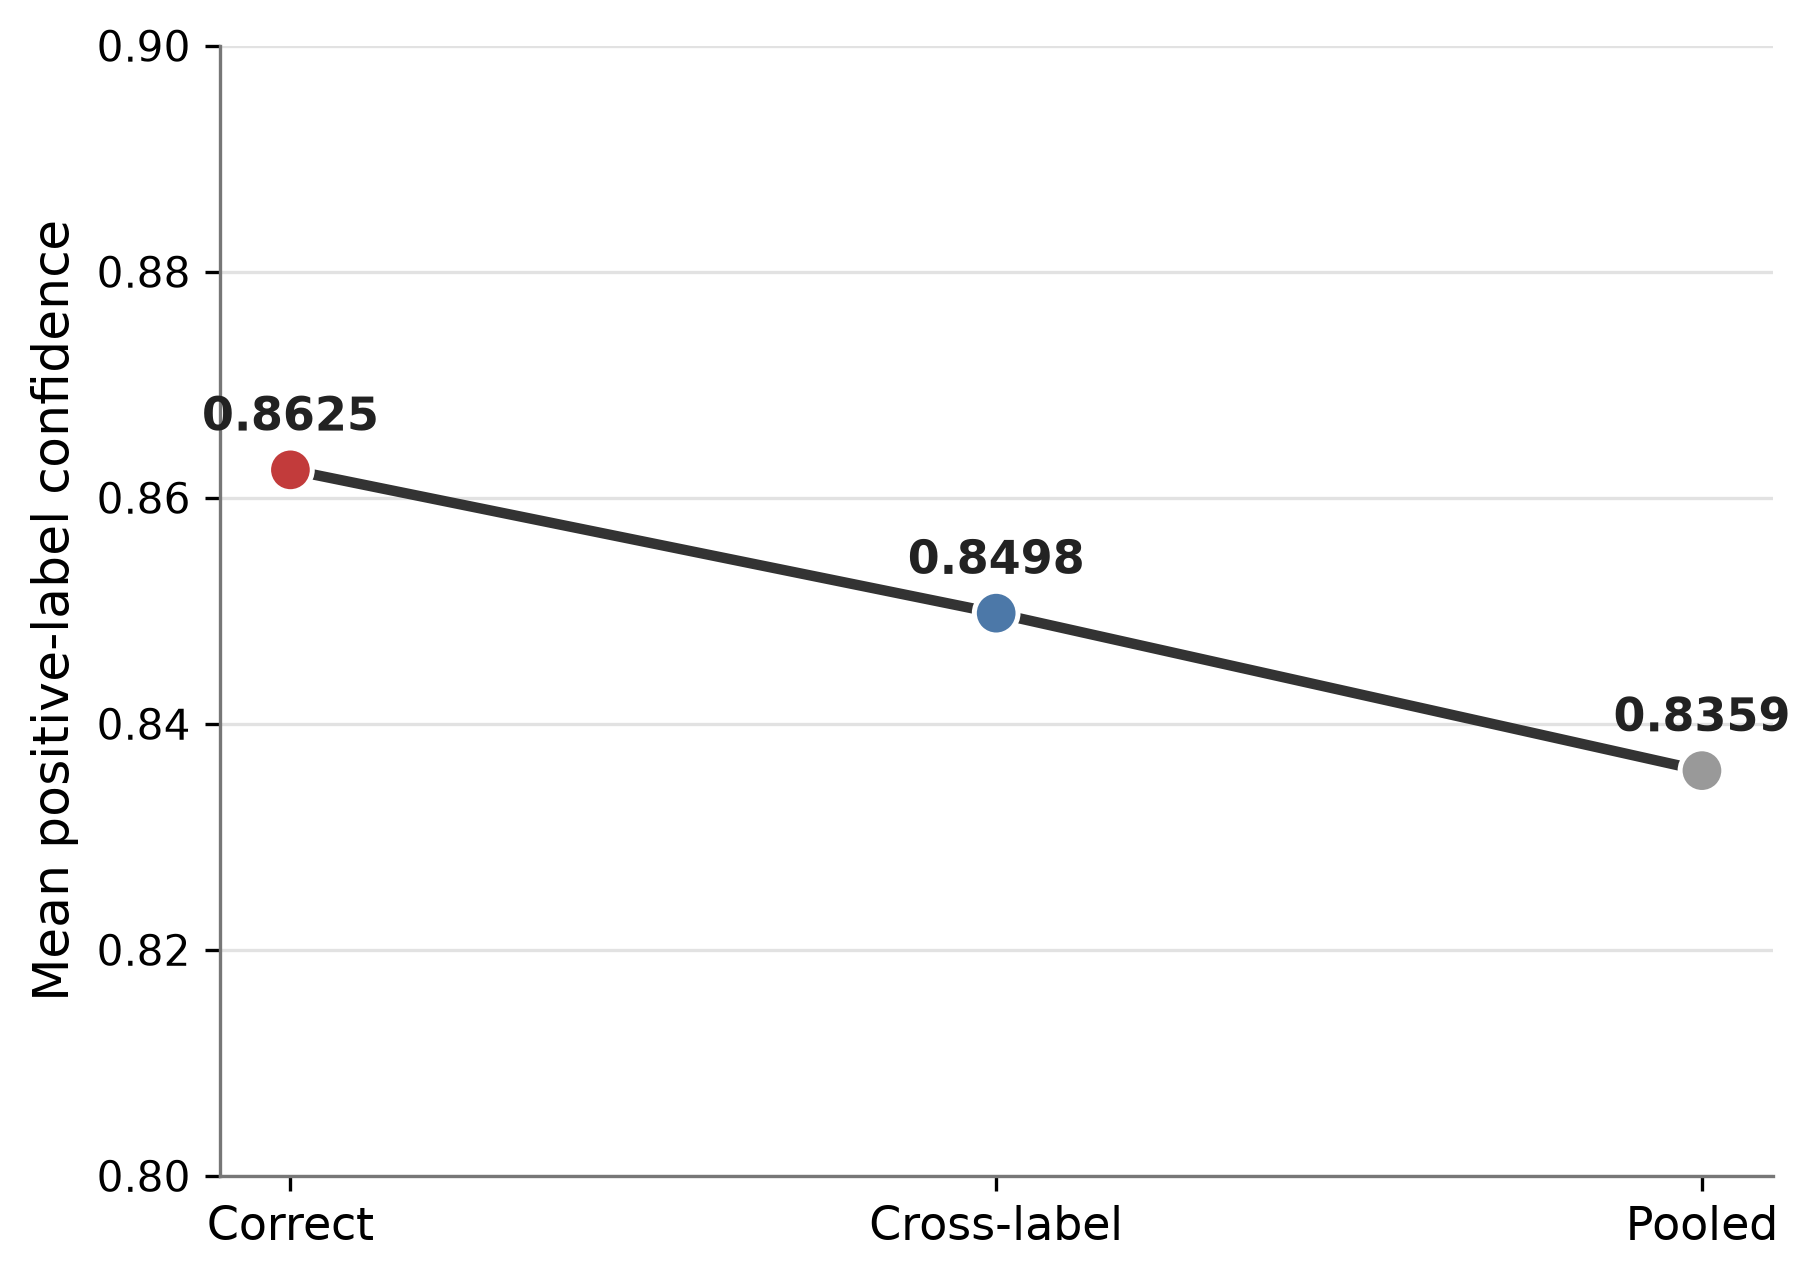
\includegraphics[width=0.62\textwidth]{figs/label_query_retrieval_specificity_four_datasets.png}
\caption{Label-specific textual retrieval analysis across the four gastroscopy datasets. Correct retains the text representation retrieved by its corresponding label query, Cross-label reassigns retrieved representations across labels, and Pooled replaces them with a shared description representation. The line shows mean confidence assigned to positive labels after combining the four datasets.\label{fig:label_query_retrieval_specificity}}
\end{figure*}

\subsubsection{Full-factorial ablation of the main architectural components}

To evaluate the individual contributions and interactions of the main architectural components, we tested all 16 combinations of APro-CoPE-based acquisition-aware Transformer context modeling, label hypergraph reasoning, label-query cross-attention, and gated residual fusion using 64 sampled images per examination. When label hypergraph reasoning was disabled, an ordinary learnable label graph was used. When both label-query cross-attention and gated residual fusion were disabled, prediction used the visual pathway; cross-attention without gated fusion was followed by direct addition, whereas gated fusion without cross-attention used a pooled finding-description representation.

In this experiment, M1 denotes APro-CoPE-based acquisition-aware Transformer context modeling, M2 denotes label hypergraph reasoning, M3 denotes label-query cross-attention, and M4 denotes gated residual fusion. The results in Table~\ref{T_factorial} show that APro-CoPE-based acquisition-aware Transformer context modeling alone changed macro F1 by less than 0.3 percentage points relative to the no-component baseline in every dataset. Label hypergraph reasoning provided consistent gains of 0.70--1.37 percentage points, whereas label-query cross-attention and gated residual fusion produced larger individual gains of 1.61--2.93 and 1.76--3.36 percentage points, respectively. The combination of label hypergraph reasoning and gated residual fusion was the strongest two-component configuration on all four datasets. Enabling all four components achieved the highest macro F1 in every dataset and improved over the no-component baseline by 2.78, 5.22, 4.51, and 3.34 percentage points on WLE, chromoscopic gastroscopy, surgical gastroscopy, and EUS, respectively.

\begin{table*}[t]
\scriptsize\tabletimes\centering
\caption{Full-factorial ablation of four main architectural components across the four gastroscopy datasets using 64 sampled images per examination. Values are macro F1 reported as mean $\pm$ standard deviation over five patient-grouped folds. M1: APro-CoPE-based acquisition-aware Transformer context modeling; M2: label hypergraph reasoning; M3: label-query cross-attention; M4: gated residual fusion. The internal position-design choices within M1 are analyzed in Table~\ref{T3_apro}.\label{T_factorial}}
\resizebox{\textwidth}{!}{%
\begin{tabular}{*{4}{c}*{4}{c}}
\hline
M1 & M2 & M3 & M4 & WLE & Chromoscopic & Surgical & EUS \\
\hline
-- & -- & -- & -- & \tresult{0.8871}{0.0124} & \tresult{0.8355}{0.0508} & \tresult{0.8005}{0.0734} & \tresult{0.8730}{0.0715} \\
$\checkmark$ & -- & -- & -- & \tresult{0.8874}{0.0134} & \tresult{0.8383}{0.0481} & \tresult{0.8000}{0.0639} & \tresult{0.8729}{0.0839} \\
-- & $\checkmark$ & -- & -- & \tresult{0.8941}{0.0134} & \tresult{0.8492}{0.0583} & \tresult{0.8110}{0.0667} & \tresult{0.8816}{0.0581} \\
-- & -- & $\checkmark$ & -- & \tresult{0.9032}{0.0115} & \tresult{0.8648}{0.0560} & \tresult{0.8252}{0.0563} & \tresult{0.8935}{0.0633} \\
-- & -- & -- & $\checkmark$ & \tresult{0.9047}{0.0135} & \tresult{0.8691}{0.0479} & \tresult{0.8304}{0.0619} & \tresult{0.8953}{0.0711} \\
$\checkmark$ & $\checkmark$ & -- & -- & \tresult{0.8907}{0.0110} & \tresult{0.8437}{0.0524} & \tresult{0.8055}{0.0600} & \tresult{0.8769}{0.0675} \\
$\checkmark$ & -- & $\checkmark$ & -- & \tresult{0.8964}{0.0107} & \tresult{0.8539}{0.0381} & \tresult{0.8149}{0.0457} & \tresult{0.8851}{0.0668} \\
$\checkmark$ & -- & -- & $\checkmark$ & \tresult{0.8981}{0.0124} & \tresult{0.8532}{0.0448} & \tresult{0.8161}{0.0621} & \tresult{0.8874}{0.0626} \\
-- & $\checkmark$ & $\checkmark$ & -- & \tresult{0.9017}{0.0119} & \tresult{0.8640}{0.0385} & \tresult{0.8236}{0.0538} & \tresult{0.8919}{0.0677} \\
-- & $\checkmark$ & -- & $\checkmark$ & \tresult{0.9063}{0.0098} & \tresult{0.8693}{0.0444} & \tresult{0.8297}{0.0450} & \tresult{0.8952}{0.0700} \\
-- & -- & $\checkmark$ & $\checkmark$ & \tresult{0.8977}{0.0141} & \tresult{0.8577}{0.0427} & \tresult{0.8201}{0.0621} & \tresult{0.8884}{0.0587} \\
$\checkmark$ & $\checkmark$ & $\checkmark$ & -- & \tresult{0.9031}{0.0128} & \tresult{0.8658}{0.0320} & \tresult{0.8267}{0.0456} & \tresult{0.8921}{0.0567} \\
$\checkmark$ & $\checkmark$ & -- & $\checkmark$ & \tresult{0.9056}{0.0119} & \tresult{0.8693}{0.0437} & \tresult{0.8299}{0.0491} & \tresult{0.8940}{0.0538} \\
$\checkmark$ & -- & $\checkmark$ & $\checkmark$ & \tresult{0.8963}{0.0135} & \tresult{0.8518}{0.0406} & \tresult{0.8166}{0.0408} & \tresult{0.8853}{0.0623} \\
-- & $\checkmark$ & $\checkmark$ & $\checkmark$ & \tresult{0.8990}{0.0107} & \tresult{0.8607}{0.0424} & \tresult{0.8223}{0.0389} & \tresult{0.8881}{0.0527} \\
$\checkmark$ & $\checkmark$ & $\checkmark$ & $\checkmark$ & \tresult{\textbf{0.9149}}{\textbf{0.0114}} & \tresult{\textbf{0.8877}}{\textbf{0.0168}} & \tresult{\textbf{0.8456}}{\textbf{0.0224}} & \tresult{\textbf{0.9064}}{\textbf{0.0474}} \\
\hline
\end{tabular}
}
\end{table*}

\FloatBarrier

\subsection{Image-only Knowledge Transfer}

To evaluate whether multimodal knowledge learned from paired images and finding descriptions could improve prediction when finding-description text was unavailable at inference, we compared four training configurations of the auxiliary image-only branch. The image-only baseline was optimized using only $\mathcal{L}_{img}$. Knowledge distillation (KD) added the prediction-level signal from the pretrained and frozen multimodal teacher, whereas multimodal branch supervision added $\mathcal{L}_{mm}$ to update the shared visual encoder. The combined configuration used both transfer mechanisms. For all four configurations, validation and test predictions were produced by the image-only branch using endoscopic images alone.

The results in Table~\ref{T_image_transfer} show that KD alone provided consistent but modest improvements over the image-only baseline, increasing macro F1 by 0.51--0.59 percentage points across the four datasets. Multimodal branch supervision produced larger gains of 1.58--1.82 percentage points. Combining KD with multimodal branch supervision achieved the strongest image-only results, improving over the baseline by 2.29--2.64 percentage points.

\begin{table*}[t]
\scriptsize\tabletimes\centering
\caption{Five-fold performance of the auxiliary image-only branch under different training-time multimodal knowledge-transfer strategies. MM sup. denotes direct supervision of the trainable multimodal branch; KD denotes knowledge distillation from a pretrained and frozen multimodal teacher. The first row uses image-only supervision without multimodal guidance. All configurations use images alone during validation and testing. Values are macro F1 reported as mean $\pm$ standard deviation over five patient-grouped folds.\label{T_image_transfer}}
\resizebox{\textwidth}{!}{%
\begin{tabular}{lcc*{4}{c}}
\hline
Model & KD & MM sup. & WLE & Chromoscopic & Surgical & EUS \\
\hline
\multirow{4}{*}{\shortstack{Image-only\\Branch}} & -- & -- & \tresult{0.8841}{0.0068} & \tresult{0.7720}{0.0645} & \tresult{0.7693}{0.0495} & \tresult{0.8527}{0.0692} \\
 & $\checkmark$ & -- & \tresult{0.8900}{0.0104} & \tresult{0.7771}{0.0542} & \tresult{0.7744}{0.0653} & \tresult{0.8583}{0.0506} \\
 & -- & $\checkmark$ & \tresult{0.9023}{0.0069} & \tresult{0.7878}{0.0870} & \tresult{0.7851}{0.0627} & \tresult{0.8702}{0.0697} \\
 & $\checkmark$ & $\checkmark$ & \tresult{\textbf{0.9105}}{\textbf{0.0120}} & \tresult{\textbf{0.7950}}{\textbf{0.0842}} & \tresult{\textbf{0.7922}}{\textbf{0.0871}} & \tresult{\textbf{0.8781}}{\textbf{0.0656}} \\
\hline
\end{tabular}
}
\end{table*}

\FloatBarrier

\section{Discussion}

Text-only models substantially outperformed image-only MIL methods on most datasets, especially on EUS. This indicates that the gastroscopic finding descriptions contain considerably more target-related information than the image sequences under examination-level weak supervision. It also raises a potential semantic label-leakage concern: although the final labels were clinically reviewed and direct category expressions were masked, descriptions of lesion morphology and location may still strongly imply the corresponding diagnosis.

The image-only transfer experiments showed that multimodal knowledge learned from paired images and finding descriptions improved visual prediction under image-only inference. Direct supervision of the trainable multimodal branch produced larger gains than knowledge distillation alone, while their combination achieved the best image-only performance on all four datasets. These results indicate that shared-encoder supervision and prediction-level distillation transfer complementary multimodal knowledge to the image-only branch.

Examination-level multimodal multi-label classification remains an emerging clinical AI task. It requires a single model to integrate multiple images acquired during one examination, learn from examination-level supervision, identify coexisting diseases, and incorporate paired clinical text. When this study was initiated, our search of the publicly available literature found no work combining these four elements within a single task. By formulating and evaluating this setting across four gastroscopy datasets, this study establishes an initial methodological basis for examination-level multimodal coexistence classification and provides a reference for analogous tasks beyond endoscopy.

\section{Conclusions}

We developed \textit{AMEF-MIL} for examination-level multi-label classification of gastroscopy examinations using ordered endoscopic image sequences and category-masked gastroscopic finding descriptions. Under patient-grouped five-fold evaluation, the primary multimodal output achieved mean macro F1 scores of 0.9149, 0.8877, 0.8456, and 0.9064 on the WLE, chromoscopic gastroscopy, surgical gastroscopy, and EUS datasets, respectively, and outperformed the compared image-only, text-only, and multimodal methods on all four datasets. The image-budget and position-component experiments showed that APro-CoPE improved the use of ordered examination images, while the full-factorial ablation supported the combined contribution of acquisition-aware context modeling, label hypergraph reasoning, label-query cross-attention, and gated residual fusion. For inference without finding-description text, multimodal branch supervision and frozen-teacher knowledge distillation both improved the auxiliary image-only branch, with their combination achieving the strongest image-only performance. Overall, this study establishes an examination-level multimodal multi-label classification paradigm that treats each examination as an integrated learning unit, jointly models multiple examination images, paired finding descriptions, and coexisting disease predictions, and provides a transferable framework for other multi-image clinical examinations.

\section*{Author contributions}

Zijian Lin conceived the study, designed the computational framework, implemented the data processing and model training pipeline, performed the experiments, analyzed the results, and drafted the manuscript. Chengze Cai contributed to model design, experimental planning, and manuscript revision. Chenxi Huang provided academic supervision and methodological guidance. Hua Gao and Jie He provided clinical supervision, data access coordination, and interpretation of clinical relevance. All authors reviewed and approved the manuscript.

\section*{ORCID iDs}
Zijian Lin \href{https://orcid.org/0009-0007-7260-4064}{0009-0007-7260-4064}\\
Chengze Cai \href{https://orcid.org/0009-0000-8851-1005}{0009-0000-8851-1005}\\
Chenxi Huang \href{https://orcid.org/0000-0002-6695-753X}{0000-0002-6695-753X}\\
Hua Gao \href{https://orcid.org/0009-0007-9844-998X}{0009-0007-9844-998X}\\
Jie He \href{https://orcid.org/0009-0000-6423-3928}{0009-0000-6423-3928}

\section*{Statements and declarations}

\subsection*{Ethical considerations}

This retrospective study used de-identified clinical archive data provided with permission from Zhongshan Hospital, Fudan University, and Zhongshan Hospital (Xiamen), Fudan University. The analysis did not use directly identifiable personal information.

\subsection*{Consent for publication}

Not applicable because no directly identifiable personal details are reported in this draft manuscript.

\begin{dci}
The author(s) declared no potential conflicts of interest with respect to the research, authorship, and/or publication of this article.
\end{dci}

\begin{funding}
This work was supported by the Natural Science Foundation of Fujian Province (No. 2025J011511).
\end{funding}

\subsection*{Data availability}

The raw gastroscopy images and clinical report data are not publicly available because they may contain sensitive clinical information and are subject to the participating hospitals' data governance requirements. De-identified derived data tables and code may be made available from the corresponding author on reasonable request and with permission from both hospitals.

\begin{acks}
The authors thank the two chief physicians from the participating hospitals for their independent clinical review of the examination-level labels.
\end{acks}

\begin{thebibliography}{99}

\bibitem{R1}
Pogorelov K, Randel KR, Griwodz C, de Lange T, Eskeland S, Johansen D, et al. Kvasir: A multi-class image dataset for computer aided gastrointestinal disease detection. In: \textit{Proceedings of the 8th ACM on Multimedia Systems Conference}. 2017, pp. 164--169.

\bibitem{R2}
Borgli H, Thambawita V, Smedsrud PH, Hicks S, Jha D, Eskeland S, et al. HyperKvasir, a comprehensive multi-class image and video dataset for gastrointestinal endoscopy. \textit{Scientific Data} 2020; 7: 283.

\bibitem{R3}
Jha D, Ali S, Hicks S, Thambawita V, Borgli H, Smedsrud PH, et al. A comprehensive analysis of classification methods in gastrointestinal endoscopy imaging. \textit{Medical Image Analysis} 2021; 70: 102007.

\bibitem{R4}
Takiyama H, Ozawa T, Ishihara S, Fujishiro M, Shichijo S, Nomura S, Miura M and Tada T. Automatic anatomical classification of esophagogastroduodenoscopy images using deep convolutional neural networks. \textit{Scientific Reports} 2018; 8: 7497.

\bibitem{R5}
Hirasawa T, Aoyama K, Tanimoto T, Ishihara S, Shichijo S, Ozawa T, et al. Application of artificial intelligence using a convolutional neural network for detecting gastric cancer in endoscopic images. \textit{Gastric Cancer} 2018; 21: 653--660.

\bibitem{R6}
Luo H, Xu G, Li C, He L, Luo L, Wang Z, et al. Real-time artificial intelligence for detection of upper gastrointestinal cancer by endoscopy: a multicentre, case-control, diagnostic study. \textit{The Lancet Oncology} 2019; 20: 1645--1654.

\bibitem{R7}
Wu L, Zhang J, Zhou W, An P, Shen L, Liu J, et al. Randomised controlled trial of WISENSE, a real-time quality improving system for monitoring blind spots during esophagogastroduodenoscopy. \textit{Gut} 2019; 68: 2161--2169.

\bibitem{R8}
Buendgens L, Cifci D, Ghaffari Laleh N, van Treeck M, Koenen MT, Zimmermann HW, et al. Weakly supervised end-to-end artificial intelligence in gastrointestinal endoscopy. \textit{Scientific Reports} 2022; 12: 4829.

\bibitem{R9}
Bravo D, Frias J, Vera F, Trejos J, Martinez C, Gomez M, et al. GastroHUN an endoscopy dataset of complete systematic screening protocol for the stomach. \textit{Scientific Data} 2025; 12: 102.

\bibitem{R10}
Ilse M, Tomczak JM and Welling M. Attention-based deep multiple instance learning. In: \textit{Proceedings of the 35th International Conference on Machine Learning}. 2018, pp. 2127--2136.

\bibitem{R11}
Lu MY, Williamson DFK, Chen TY, Chen RJ, Barbieri M and Mahmood F. Data-efficient and weakly supervised computational pathology on whole-slide images. \textit{Nature Biomedical Engineering} 2021; 5: 555--570.

\bibitem{R12}
Li B, Li Y and Eliceiri KW. Dual-stream multiple instance learning network for whole slide image classification with self-supervised contrastive learning. In: \textit{Proceedings of the IEEE/CVF Conference on Computer Vision and Pattern Recognition}. 2021, pp. 14318--14328.

\bibitem{R13}
Shao Z, Bian H, Chen Y, Wang Y, Zhang J, Ji X, et al. TransMIL: Transformer based correlated multiple instance learning for whole slide image classification. In: \textit{Advances in Neural Information Processing Systems}. 2021.

\bibitem{R14}
Zhang H, Meng Y, Zhao Y, Qiao Y, Yang X, Coupland SE and Zheng Y. DTFD-MIL: Double-tier feature distillation multiple instance learning for histopathology whole slide image classification. In: \textit{Proceedings of the IEEE/CVF Conference on Computer Vision and Pattern Recognition}. 2022, pp. 18802--18812.

\bibitem{R15}
Campanella G, Hanna MG, Geneslaw L, Miraflor A, Silva VWK, Busam KJ, et al. Clinical-grade computational pathology using weakly supervised deep learning on whole slide images. \textit{Nature Medicine} 2019; 25: 1301--1309.

\bibitem{R16}
Ridnik T, Ben-Baruch E, Zamir N, Noy A, Friedman I, Protter M and Zelnik-Manor L. Asymmetric loss for multi-label classification. In: \textit{Proceedings of the IEEE/CVF International Conference on Computer Vision}. 2021, pp. 82--91.

\bibitem{R17}
Chen ZM, Wei XS, Wang P and Guo Y. Multi-label image recognition with graph convolutional networks. In: \textit{Proceedings of the IEEE/CVF Conference on Computer Vision and Pattern Recognition}. 2019, pp. 5177--5186.

\bibitem{R18}
Feng Y, You H, Zhang Z, Ji R and Gao Y. Hypergraph neural networks. In: \textit{Proceedings of the AAAI Conference on Artificial Intelligence}. 2019; 33: 3558--3565.

\bibitem{R19}
Li J, Selvaraju RR, Gotmare AD, Joty S, Xiong C and Hoi SCH. Align before fuse: Vision and language representation learning with momentum distillation. In: \textit{Advances in Neural Information Processing Systems}. 2021.

\bibitem{R20}
Li J, Li D, Xiong C and Hoi S. BLIP: Bootstrapping language-image pre-training for unified vision-language understanding and generation. In: \textit{Proceedings of the International Conference on Machine Learning}. 2022.

\bibitem{R21}
Zhang Y, Jiang H, Miura Y, Manning CD and Langlotz CP. Contrastive learning of medical visual representations from paired images and text. In: \textit{Proceedings of Machine Learning Research}. 2022; 182: 1--24.

\bibitem{R22}
Huang SC, Shen L, Lungren MP and Yeung S. GLoRIA: A multimodal global-local representation learning framework for label-efficient medical image recognition. In: \textit{Proceedings of the IEEE/CVF International Conference on Computer Vision}. 2021, pp. 3942--3951.

\bibitem{R23}
Zhou HY, Chen X, Zhang Y, Luo R, Wang L and Yu Y. Generalized radiograph representation learning via cross-supervision between images and free-text radiology reports. \textit{Nature Machine Intelligence} 2022; 4: 32--40.

\bibitem{R24}
Hinton G, Vinyals O and Dean J. Distilling the knowledge in a neural network. \textit{arXiv preprint arXiv:1503.02531} 2015.

\bibitem{R25}
Lopez-Paz D, Bottou L, Schölkopf B and Vapnik V. Unifying distillation and privileged information. In: \textit{International Conference on Learning Representations}. 2016.

\bibitem{R26}
Vaswani A, Shazeer N, Parmar N, Uszkoreit J, Jones L, Gomez AN, et al. Attention is all you need. In: \textit{Advances in Neural Information Processing Systems}. 2017.

\bibitem{R27}
Golovneva O, Wang T, Weston J and Sukhbaatar S. Contextual position encoding: Learning to count what's important. \textit{arXiv preprint arXiv:2405.18719} 2024.

\bibitem{R28}
Liu Z, Mao H, Wu CY, Feichtenhofer C, Darrell T and Xie S. A ConvNet for the 2020s. In: \textit{Proceedings of the IEEE/CVF Conference on Computer Vision and Pattern Recognition}. 2022, pp. 11976--11986.

\bibitem{R29}
Zhu X, Qian P, Wang C, Liu L, Gao M, Cai W and Ng EYK. MMFNet: A multi-modal and multi-attention fusion network for multi-task skin disease classification. In: \textit{2024 IEEE International Conference on Bioinformatics and Biomedicine}. 2024, pp. 1779--1782.

\bibitem{R30}
Zhang J, He K, Feng Z, Sun S, Sun X, Yuan Z and Yu J. Self-adaptive image-text fusion for medical image classification. \textit{Pattern Recognition} 2025; 167: 111715.

\bibitem{R31}
Zhong D, Li X, Huang Z, Wang S, Yu Z, Hou M, et al. Multi-modal multi-scale representation learning via cross-attention between chest radiology images and free-text reports. \textit{Biomedical Signal Processing and Control} 2026; 111: 108318.

\bibitem{R32}
Jahanian M, Karimi A, Eraghi NO and Zarafshan F. Multimodal transformers for joint diagnosis and retrieval from chest X-rays and radiology reports. \textit{Informatics in Medicine Unlocked} 2025; 58: 101672.

\end{thebibliography}

\end{document}
